% ============================================================
%  Chapter 7 – Stochastic Optimization
%  Lectures on Monte Carlo Theory – Lorek & Rolski
%  Reader-friendly rewrite: complete sentences, worked examples,
%  all symbols defined, Greek letters pronounced, allowframebreaks.
% ============================================================
\documentclass[aspectratio=169,10pt]{beamer}
\usetheme{Madrid}
\usecolortheme{seahorse}
\setbeamertemplate{footline}[frame number]
\usefonttheme[onlymath]{serif}

% -- packages ------------------------------------------------
\usepackage{amsmath,amssymb,mathtools}
\usepackage{bm}
\usepackage{graphicx}
\usepackage{booktabs}
\usepackage{listings}
\usepackage{xcolor}
\usepackage{algorithm}
\usepackage{algpseudocode}
\usepackage{tikz}
\usepackage{enumerate}
\usepackage{array}

\graphicspath{{figures/}}

% -- listings style ------------------------------------------
\lstdefinestyle{python}{
  language=Python,
  basicstyle=\ttfamily\scriptsize,
  numbers=left,
  numberstyle=\tiny\color{gray},
  frame=single,
  backgroundcolor=\color{gray!7},
  keywordstyle=\color{blue!70!black}\bfseries,
  commentstyle=\color{green!50!black}\itshape,
  stringstyle=\color{orange!80!black},
  breaklines=true,
  showstringspaces=false,
  tabsize=4,
}

% -- macros --------------------------------------------------
\newcommand{\R}{\mathbb{R}}
\newcommand{\E}{\mathbb{E}}
\newcommand{\Prob}{\mathbb{P}}
\newcommand{\bx}{\mathbf{x}}
\newcommand{\bv}{\mathbf{v}}
\newcommand{\bw}{\mathbf{w}}
\newcommand{\btheta}{\boldsymbol{\theta}}
\newcommand{\calS}{\mathcal{S}}
\newcommand{\calE}{\mathcal{E}}
\newcommand{\calN}{\mathcal{N}}
\newcommand{\ind}[1]{\mathbf{1}\!\left(#1\right)}

% ============================================================
\title[Ch.7 Stochastic Optimization]{Chapter 7\\Stochastic Optimization}
\subtitle{Lectures on Monte Carlo Theory}
\author{Lorek \& Rolski}
\date{}
% ============================================================

\begin{document}

% -- Title ---------------------------------------------------
\begin{frame}
  \titlepage
\end{frame}

% -- Outline -------------------------------------------------
\begin{frame}{Chapter Outline}
  \tableofcontents
\end{frame}

% ============================================================
\section{Introduction: The Stochastic Optimization Problem}
% ============================================================

\begin{frame}[allowframebreaks]{Introduction: The Stochastic Optimization Problem}

In this chapter we study Monte Carlo methods for a fundamental class of
real-world problems: given a function $h : \calS \to \R$ (read: ``$h$ maps
the set $\calS$ to the real numbers $\R$'') defined on some set $\calS$
(script S, the \textbf{solution space} or \textbf{state space}), we want to
find both the maximum value and the argument that achieves it.

\begin{block}{The Optimization Objective}
  \[
    \gamma^{\mathrm{opt}} = \max_{x \in \calS} h(x),
    \qquad
    x^{\mathrm{opt}} = \arg\max_{x \in \calS} h(x).
  \]
  \textbf{Notation:} $\calS$ is the solution space (possibly combinatorial
  and enormous), $h$ is the \textbf{performance function} whose maximum we
  seek, $\gamma^{\mathrm{opt}}$ (gamma, pronounced ``gamma'', superscript
  ``opt'' for optimal) is the best achievable value, and $x^{\mathrm{opt}}$
  is the solution that achieves it.  The symbol $\max_{x \in \calS}$ means
  ``the largest value of $h(x)$ over all choices of $x$ in $\calS$'', and
  $\arg\max$ means ``the $x$ that gives that largest value''.
\end{block}

\begin{alertblock}{How to Read This}
  This formula simply asks: among all possible solutions $x$ in the space
  $\calS$, which one makes $h(x)$ as large as possible, and what is that
  largest value?  When we want to \emph{minimise} a cost function
  $H : \calS \to \mathbb{R}_+$ instead, we set $h = -H$, and the minimiser
  of $H$ is the same as the maximiser of $-H$.  All maximisation algorithms
  in this chapter therefore apply directly to minimisation problems too.
\end{alertblock}

\medskip
\textbf{Why can we not just check every solution?}
For small $\calS$ one can evaluate $h$ at every point and return the
maximum.  But for combinatorial spaces the size of $\calS$ is astronomically
large:
\begin{itemize}
  \item All tours of $n = 20$ cities: $20! \approx 2.4 \times 10^{18}$ --- at
    $10^9$ evaluations per second this would take about \textbf{76 years}.
  \item All binary vectors of length $d = 100$: $2^{100} \approx 10^{30}$
    --- completely infeasible.
\end{itemize}
The key insight of stochastic optimisation is to \emph{search intelligently}
rather than exhaustively, by building a random process that naturally
gravitates toward the optimum.

\framebreak

\textbf{The Boltzmann bridge: connecting probability and optimisation.}

The Boltzmann distribution (named after physicist Ludwig Boltzmann,
1844--1906) provides the theoretical bridge between probability theory and
optimisation.  For a cost function $H$ and a temperature parameter $T > 0$
(where $T$ is a positive real number controlling how much randomness to
allow), define the probability assigned to each solution $v$ in the solution
set $V$ as:
\[
  \pi^T_v \;\propto\; e^{-H(v)/T}, \qquad v \in V.
\]
The symbol $\propto$ (read ``proportional to'') means the right-hand side is
divided by a normalising constant so that all probabilities sum to one.

\begin{block}{Notation for the Boltzmann Distribution}
  $\pi^T_v$ (pi, pronounced ``pie'', superscript $T$, subscript $v$) is
  the probability assigned to solution $v$ at temperature $T$.  $H(v)$ is
  the cost (how bad solution $v$ is).  $e^{-H(v)/T}$ (e to the negative
  H-of-v divided by T) is the Boltzmann weight: it is large when $H(v)$ is
  small (good solution) and small when $H(v)$ is large (bad solution).  As
  $T \to 0$ (temperature goes to zero), all probability mass concentrates on
  the minimiser(s) of $H$.
\end{block}

\textbf{Five methods covered in this chapter.}
The five stochastic optimisation methods form a natural progression in
sophistication:

\begin{enumerate}
  \item \textbf{Metropolis at fixed temperature.}  Run a Markov chain whose
    stationary distribution is the Boltzmann distribution $\pi^T$ at a fixed
    $T > 0$.  Simple, but can be trapped in local minima.

  \item \textbf{Simulated Annealing (SA).}  Gradually decrease
    $T_k \searrow 0$ ($T$ sub $k$ decreases toward zero following a cooling
    schedule).  At high temperatures the chain explores freely; as
    $T_k \to 0$ it converges to the global minimum.  With slow enough
    cooling the convergence is guaranteed by the celebrated Haj\'{e}k theorem.

  \item \textbf{Locally Informed Proposals (LIP).}  Rather than proposing a
    uniformly random neighbour, evaluate the Boltzmann weights of multiple
    candidate neighbours and propose with probability proportional to their
    quality.  The chain still targets $\pi^T$ exactly (via a
    Metropolis--Hastings correction) but moves in productive directions far
    more often.

  \item \textbf{Cross-Entropy (CE) method.}  Maintain a \emph{parametric
    distribution} $p_{\btheta}$ (p sub theta) over all of $\calS$ and
    iteratively update the parameter $\btheta$ (theta, pronounced ``thay-ta'')
    so that $p_{\btheta}$ concentrates on the best-performing solutions.

  \item \textbf{Metropolis--CE hybrid.}  Combine the local Markov-chain
    walk of Metropolis with the distributional parameter learning of CE,
    inheriting the best of both approaches.
\end{enumerate}

\framebreak

\textbf{Two running benchmark problems.}

All five methods are compared on two standard combinatorial optimisation
problems that together stress-test every algorithm.

\begin{block}{Travelling Salesman Problem (TSP)}
  Given $n$ cities with symmetric distance matrix $\mathbf{M}$ (entry
  $M(i,j) = M(j,i)$ = distance from city $i$ to city $j$), find the
  permutation $\sigma^*$ (sigma, a complete tour visiting all cities exactly
  once) in the set $\mathcal{S}_n$ of all $n!$ permutations that minimises
  the total tour length:
  \[
    l(\sigma) = \sum_{k=1}^{n-1}\mathbf{M}(\sigma(k),\sigma(k+1))
      + \mathbf{M}(\sigma(n),\sigma(1)).
  \]
  Here $\sigma(k)$ is the $k$-th city visited, and the final term
  $\mathbf{M}(\sigma(n),\sigma(1))$ is the return leg to the starting city.
  For our 13-city USA benchmark: optimal tour length is \textbf{7024 miles};
  a uniformly random tour has expected length $\approx 15938$ miles --- more
  than twice as long.
\end{block}

\begin{block}{0-1 Knapsack Problem}
  Given $d$ items with weights $\bw = (w_1,\ldots,w_d)$ and values
  $\bv = (v_1,\ldots,v_d)$ and a weight capacity $W$, choose a binary
  vector $\bx \in \{0,1\}^d$ (each $x_i \in \{0,1\}$ decides whether item
  $i$ is included) to
  \[
    \text{maximise} \quad f(\bx) = \bv\cdot\bx = \sum_{i=1}^d v_i x_i
    \quad \text{subject to} \quad \bw\cdot\bx = \sum_{i=1}^d w_i x_i \le W.
  \]
  Here $\Sigma$ (Sigma, meaning ``sum'') over $i$ from 1 to $d$ adds up the
  values (or weights) of all included items.  Our benchmark: $d=100$,
  $w_i=i$, $v_i=i^{1.2}$, $W=3000$.
\end{block}

\begin{alertblock}{Key Insight}
  All five methods share one unifying idea: build a probability distribution
  that is higher on better solutions, then use Monte Carlo techniques to
  locate the distribution's mode (the highest-probability solution).  The
  methods differ in \emph{how} they construct and sample from this
  distribution efficiently.
\end{alertblock}

\end{frame}

% ============================================================
\section{7.1 Metropolis and Gibbs Based Methods}
% ============================================================

\begin{frame}[allowframebreaks]{7.1 Metropolis and Gibbs Based Methods: Setup}

We work with a graph $G = (V, E)$ where $V$ is the set of candidate
solutions and each edge connects two \emph{neighbouring} solutions (solutions
reachable by one local move).  We are given a cost function
$H : V \to \mathbb{R}_+$ (H maps V to the non-negative reals) and want to
find $v^* = \arg\min_{v \in V} H(v)$ --- the solution with minimum cost.

\medskip
\textbf{The Boltzmann distribution: putting more probability on better solutions.}
The core idea is to construct a probability distribution on $V$ that assigns
higher probability to states with lower cost.  The \emph{Boltzmann
distribution} at temperature $T > 0$ does exactly this:

\begin{block}{Boltzmann Distribution (Eq.~7.1.1)}
  \[
    \pi^T_v = \frac{e^{-H(v)/T}}{\displaystyle\sum_{v' \in V} e^{-H(v')/T}},
    \qquad v \in V, \quad T > 0.
  \]
  \textbf{Notation:} $\pi^T_v$ (pi superscript $T$, subscript $v$) is the
  probability of solution $v$ at temperature $T$.  $H(v) \ge 0$ is the cost
  of solution $v$.  $e^{-H(v)/T}$ is the Boltzmann weight of $v$ --- it is
  close to 1 when $H(v)$ is small (good solution) and close to 0 when
  $H(v)$ is large (bad solution).  The denominator
  $\sum_{v' \in V} e^{-H(v')/T}$ is the \emph{partition function} --- the
  normalising constant that makes all probabilities sum to one.
\end{block}

\begin{alertblock}{How to Read This Formula}
  Think of the temperature $T$ as a dial.  When $T$ is very large (dial
  turned up), the exponent $-H(v)/T$ is close to zero for every $v$, so all
  Boltzmann weights $e^{-H(v)/T} \approx 1$ and the distribution is nearly
  uniform --- the chain wanders everywhere.  When $T$ is very small (dial
  turned down), even tiny differences in cost are magnified: a solution with
  cost 3 gets weight $e^{-3/0.01} \approx 10^{-130}$ while a solution with
  cost 2 gets weight $e^{-2/0.01} \approx 10^{-87}$ --- a ratio of $10^{43}$
  to 1.  In the limit $T \to 0$, only the lowest-cost solution has non-zero
  probability.
\end{alertblock}

The key observation is that the Boltzmann distribution's mode is exactly the
minimiser of $H$, regardless of the temperature $T > 0$:
\[
  \arg\min_{v \in V} H(v) \;=\; \arg\max_{v \in V} \pi^T_v \quad
  \text{for any } T > 0.
\]
Therefore, if we can sample from $\pi^T$ and identify the most frequently
visited state, we have found the optimum.  When we want to \emph{maximise}
a function $f : V \to \mathbb{R}_+$, we set $H(v) = -f(v)$, giving
$\pi^T_v \propto e^{f(v)/T}$, which concentrates on the maximiser of $f$.

\framebreak

\textbf{The Metropolis--Hastings algorithm for $\pi^T$.}
To sample from $\pi^T$ via MCMC we apply Metropolis--Hastings with a simple
random walk on $G$ as the proposal: from state $v$, propose a uniformly
random neighbour $v'$ (so the proposal probability is
$q_{vv'} = 1/\deg(v)$ for each $v' \in \calN(v)$, where $\deg(v)$ denotes
the degree of $v$, i.e., the number of neighbours, and $\calN(v)$ denotes
the set of neighbours).  The Metropolis--Hastings acceptance probability is:

\begin{block}{Acceptance Probability (Algorithm 61)}
  \[
    \alpha^T_{vv'} = \min\!\left(1,\;
      \frac{\pi^T_{v'} q_{v'v}}{\pi^T_v q_{vv'}}
    \right)
    = \min\!\left(1,\;
      \frac{\deg(v)}{\deg(v')}\cdot
      e^{(H(v)-H(v'))/T}
    \right),
    \quad v,v' \in V.
  \]
  \textbf{Notation:} $\alpha^T_{vv'}$ (alpha, pronounced ``al-fa'') is the
  probability of accepting the proposed move from $v$ to $v'$.
  $\deg(v)/\deg(v')$ is the ratio of the number of neighbours of $v$ to the
  number of neighbours of $v'$; this equals 1 for regular graphs.
  $e^{(H(v)-H(v'))/T}$ is the Boltzmann ratio: when $H(v) > H(v')$ (i.e.,
  $v'$ is better), the exponent is positive and the ratio exceeds 1, so the
  move is always accepted.
\end{block}

\begin{alertblock}{How to Read the Acceptance Rule}
  A move to a \emph{better} solution ($H(v') < H(v)$, lower cost) makes
  $H(v) - H(v') > 0$, so $e^{(H(v)-H(v'))/T} > 1$ and the move is
  \emph{always} accepted (the $\min$ with 1 kicks in).  A move to a
  \emph{worse} solution ($H(v') > H(v)$) makes the exponent negative, so
  acceptance probability is $e^{(H(v)-H(v'))/T} \in (0,1)$ --- we
  occasionally accept worse moves.  This occasional acceptance of worse
  moves is precisely what prevents the chain from being permanently trapped
  in a local minimum.
\end{alertblock}

The resulting transition probability from $v$ to neighbour $v'$ is:
\[
  p^T_{vv'} = \frac{1}{\deg(v)}\min\!\left(1,\;
    \frac{\deg(v)}{\deg(v')}\cdot
    e^{(H(v)-H(v'))/T}
  \right), \qquad v' \in \calN(v).
\]

\begin{exampleblock}{Worked Example: Two-State Space}
  Suppose $V = \{A, B\}$ with costs $H(A) = 2$, $H(B) = 5$, temperature
  $T = 1$, and the graph has only the edge $A$--$B$.  Both states have
  degree 1, so the degree ratio is 1.\\[4pt]
  \textbf{From $B$ (worse state), proposing move to $A$ (better):}
  $\alpha = \min(1,\, e^{(5-2)/1}) = \min(1, e^3) = 1$.  The move to the
  better state is always accepted.\\[4pt]
  \textbf{From $A$ (better state), proposing move to $B$ (worse):}
  $\alpha = \min(1,\, e^{(2-5)/1}) = e^{-3} \approx 0.050$.  Only 5\% of
  the time does the chain move to the worse state.\\[4pt]
  \textbf{Verification:} the stationary distribution is
  $\pi^T_A = e^{-2}/(e^{-2}+e^{-5}) \approx 0.953$ and
  $\pi^T_B \approx 0.047$, confirming the chain spends about 95\% of its
  time at the better solution $A$.
\end{exampleblock}

\framebreak

\begin{center}
  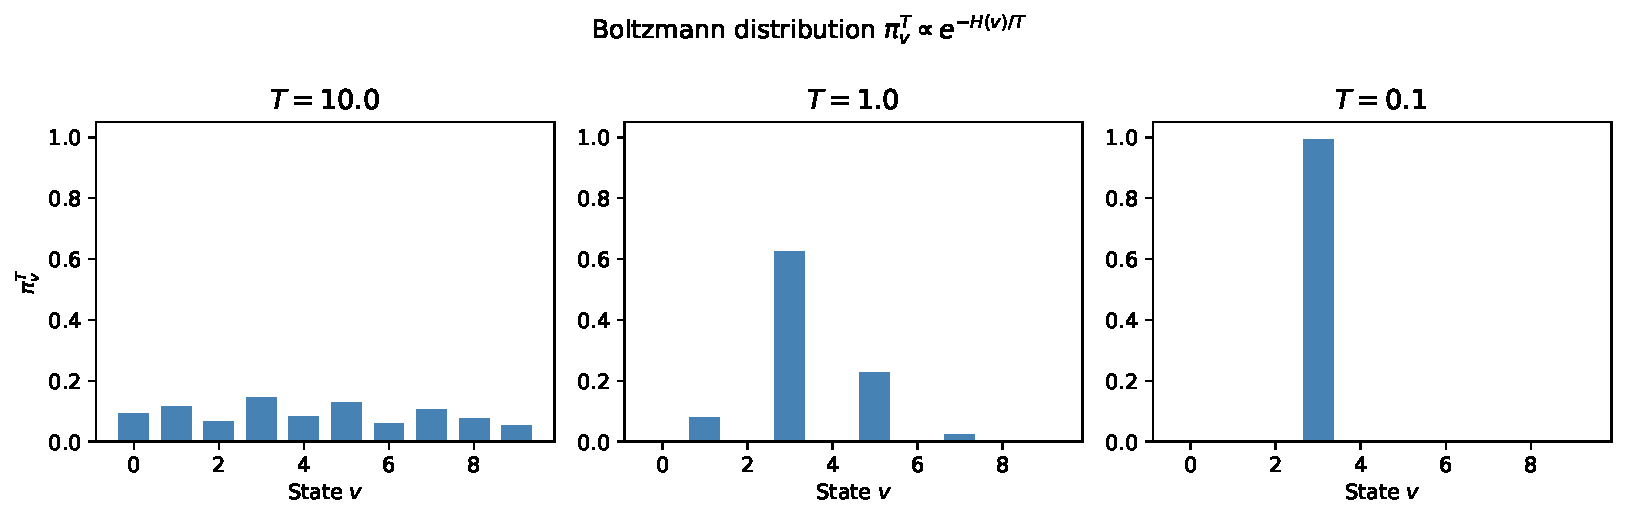
\includegraphics[width=0.78\textwidth]{fig_boltzmann}
\end{center}
{\small \textbf{Figure: Boltzmann distribution for different temperatures.}
At high temperature $T$, all states receive nearly equal probability (flat
distribution) and the chain explores freely.  As $T$ decreases, the
distribution sharpens and concentrates around the state with the smallest
cost $H(v)$.  In the limit $T \to 0$, the Boltzmann distribution becomes a
point mass (probability 1) on the global minimiser.  Fixed-temperature
Metropolis samples from $\pi^T$ for one chosen $T$, trading off exploration
(high $T$, but optimum unclear) against exploitation (low $T$, but chain
gets stuck).}

\end{frame}

\begin{frame}[allowframebreaks]{Application: Decrypting a Substitution Cipher}

A \textbf{substitution cipher} replaces each letter in the original message
(plaintext) with a different letter according to a fixed permutation
$\sigma : \Sigma \to \Sigma$, where $\Sigma$ (capital Sigma, the Greek
letter used here for the 26-letter alphabet) $= \{a, b, \ldots, z\}$.  The
ciphertext $c_1 c_2 \cdots c_L$ is produced letter by letter; to decrypt, we
need to recover $\sigma$ (sigma, pronounced ``sig-ma'').

The solution space is $\calS = \mathcal{S}_{26}$ (all permutations of 26
letters), with $26! \approx 4 \times 10^{26}$ elements --- completely
infeasible for exhaustive search.

\medskip
\textbf{The score function: bigram log-likelihood.}
English text has characteristic two-letter (bigram) frequencies.  For
example, ``th'' and ``he'' are very common while ``xz'' is vanishingly rare.
Let $\mathbf{M}(a,b)$ be the frequency with which letter $b$ follows letter
$a$ in a reference English corpus (here: Tolstoy's \emph{War and Peace}).
For a candidate decryption key $\sigma$, the log-likelihood that the
decrypted text is English is:

\begin{block}{Log-Likelihood Score (Eq.~7.1.2)}
  \[
    l(\sigma) = \sum_{i=1}^{L-1} \log \mathbf{M}(\sigma(c_i),\,\sigma(c_{i+1})).
  \]
  \textbf{Notation:} $l(\sigma)$ (lowercase $l$, the log-likelihood) is a
  real number measuring how ``English-like'' the decrypted message is under
  key $\sigma$.  $c_i$ is the $i$-th ciphertext letter.  $\sigma(c_i)$ is
  the candidate plaintext letter that the key $\sigma$ maps $c_i$ to.
  $\mathbf{M}(\sigma(c_i), \sigma(c_{i+1}))$ is the reference corpus
  frequency of the bigram $\sigma(c_i)\sigma(c_{i+1})$.  $\log$ is the
  natural logarithm.  The $\sum$ (Sigma, meaning ``sum'') runs $i$ from 1
  to $L-1$, covering all consecutive letter pairs in the ciphertext.
\end{block}

\begin{alertblock}{How to Read This Formula}
  A larger $l(\sigma)$ means the decrypted message looks more like English.
  Taking the logarithm converts a product of bigram probabilities into a
  sum, which is numerically stable (products of many small probabilities
  underflow to zero on a computer).  We set the target distribution
  $\pi_\sigma \propto e^{l(\sigma)}$, so better-looking decryptions have
  higher probability.
\end{alertblock}

\textbf{Proposal distribution.}  From permutation $\sigma$ (sigma), propose
$\sigma'$ (sigma prime) by swapping two uniformly chosen letters
$a, b \in \{1,\ldots,26\}$ (a transposition).  There are
$\binom{26}{2} = 325$ possible transpositions, each proposed with
probability $q_{\sigma\sigma'} = 1/325$.  Since the proposal is symmetric
and the graph is regular, the acceptance ratio simplifies to:
\[
  \alpha = \min\!\left(1,\; e^{l(\sigma')-l(\sigma)}\right).
\]
Crucially, this ratio requires only the \emph{change} in log-likelihood due
to the transposition --- the intractable normalising constant
$z = \sum_\sigma e^{l(\sigma)}$ cancels out completely.

\framebreak

\textbf{Simulation results for the substitution cipher.}
The algorithm was run for 3000 steps starting from a random permutation,
with the ciphertext taken from Tolstoy's \emph{Anna Karenina}.

\begin{columns}
  \column{0.56\textwidth}
  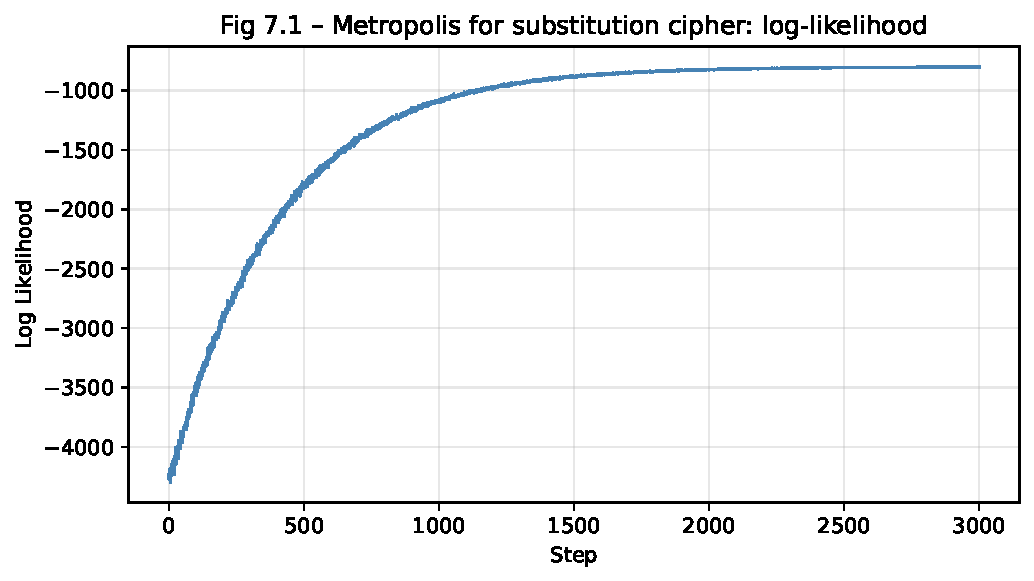
\includegraphics[width=\textwidth]{fig_cipher_loglik}
  \column{0.42\textwidth}
  \small
  \textbf{Table 7.1: Log-likelihood evolution.}\\[4pt]
  \begin{tabular}{r|r}
    \toprule
    Step & Log-likelihood\\
    \midrule
    1    & $-4274.98$\\
    1000 & $-896.09$\\
    2000 & $-826.07$\\
    3000 & $-815.71$\\
    \bottomrule
  \end{tabular}\\[6pt]
  The log-likelihood improves by \textbf{3459} units in 3000 steps.
  After step 3000 the message is recognisable English with only a few
  letters incorrect.
\end{columns}

\medskip
The curve shows a rapid climb in the first few hundred steps (rough
structure of the key found quickly) followed by a slow refinement phase
(fine-tuning individual letter swaps).  This two-phase behaviour is typical
of MCMC-based optimisation.

\begin{alertblock}{Key Insight: Computing Without the Normalising Constant}
  Metropolis works on the substitution cipher because the target
  distribution's ratio $\pi_{\sigma'}/\pi_\sigma = e^{l(\sigma')-l(\sigma)}$
  can be computed cheaply \emph{without} knowing the intractable normalising
  constant $z$.  Only the \emph{change} in log-likelihood matters.  This
  ``ratio trick'' is a recurring theme in MCMC-based optimisation: we never
  need to evaluate $z$, only the relative probability of two neighbouring
  states.
\end{alertblock}

\end{frame}

\begin{frame}[allowframebreaks]{The 0-1 Knapsack Problem: Gibbs and Metropolis}

We want to find $\bx \in \{0,1\}^d$ that maximises the total value
$f(\bx) = \bv \cdot \bx = \sum_i v_i x_i$ subject to the weight constraint
$\bw \cdot \bx = \sum_i w_i x_i \le W$.  We model this as sampling from a
Boltzmann distribution that assigns zero probability to infeasible solutions
(those that violate the weight constraint).

\begin{block}{Boltzmann Distribution for the Knapsack}
  \[
    \pi_{\bx} = \begin{cases}
      \dfrac{\exp(\bv\cdot\bx / T)}{z_T} & \text{if } \bw\cdot\bx \le W\\[8pt]
      0 & \text{if } \bw\cdot\bx > W
    \end{cases}
  \]
  \textbf{Notation:} $T > 0$ is the temperature, $z_T$ is the normalising
  constant, and $\bv \cdot \bx = \sum_i v_i x_i$ (the dot product of value
  vector $\bv$ and binary selection vector $\bx$) is the total value of
  selected items.  States violating the weight constraint have zero
  probability and are never visited.  As $T \to 0$, all mass concentrates
  on the highest-value feasible solution.
\end{block}

\medskip
\textbf{Gibbs sampler (Algorithm 63).}
The Gibbs sampler picks a random coordinate $i \in \{1,\ldots,d\}$ and
resamples $x_i$ from its conditional distribution given all other
coordinates $\bx_{-i} = (x_1,\ldots,x_{i-1},x_{i+1},\ldots,x_d)$.  The
ratio of Boltzmann weights for $x_i = 1$ versus $x_i = 0$ is $e^{v_i/T}$
(since only the $i$-th term $v_i x_i$ differs).  Therefore the conditional
probability of including item $i$ takes the familiar \emph{logistic} form:
\[
  \Prob(Z(i)=1 \mid Z_{-i}=\bx_{-i})
  = \frac{e^{v_i/T}}{1 + e^{v_i/T}}
  = \frac{1}{1 + e^{-v_i/T}},
\]
provided adding item $i$ is feasible.  If adding item $i$ would exceed
capacity we are forced to set $x_i = 0$.  This conditional is a logistic
(sigmoid) function of $v_i/T$ (v sub i divided by T): items with a higher
value-to-temperature ratio are more likely to be included.

\begin{exampleblock}{Worked Example: Gibbs Conditional Probabilities}
  Suppose temperature $T = 1$.  Then:
  \begin{itemize}
    \item $v_i = 10$: $\Prob(x_i=1) = 1/(1+e^{-10}) \approx 0.99995$.
      Almost certainly included (if feasible).
    \item $v_i = 2$: $\Prob(x_i=1) = 1/(1+e^{-2}) \approx 0.880$.
      Likely included.
    \item $v_i = 0.5$: $\Prob(x_i=1) = 1/(1+e^{-0.5}) \approx 0.622$.
      More likely included than not, but uncertain.
    \item $v_i = 0.1$: $\Prob(x_i=1) = 1/(1+e^{-0.1}) \approx 0.525$.
      Nearly 50--50.
  \end{itemize}
  The Gibbs sampler therefore has a built-in tendency to include high-value
  items, even without any explicit greedy logic.
\end{exampleblock}

\framebreak

\textbf{Metropolis algorithm for Knapsack (Algorithm 64).}
Define the neighbours of $\bx$ as all binary vectors that differ in exactly
one coordinate (single bit-flips).  Propose $\bx'$ by flipping a uniformly
random bit $i$.  When $x_i = 0$ (we are proposing to \emph{add} item $i$):
the acceptance probability is $\min(1, e^{v_i/T}) = 1$ --- adding an item
is always accepted if feasible, because the Boltzmann weight of the new
state is at least as large.  When $x_i = 1$ (we are proposing to
\emph{remove} item $i$): the acceptance probability is
$e^{-v_i/T} < 1$ --- the chain resists removing valuable items, with more
resistance at lower temperatures.

If the proposed state $\bx'$ violates the weight constraint, the move is
rejected with probability 1 (acceptance probability $= 0$).

\medskip
\textbf{Simulation results} for $d=100$, $w_i = i$, $v_i = i^{1.2}$,
$W = 3000$, $T = 1$, running for 150 steps:

\begin{columns}
  \column{0.54\textwidth}
  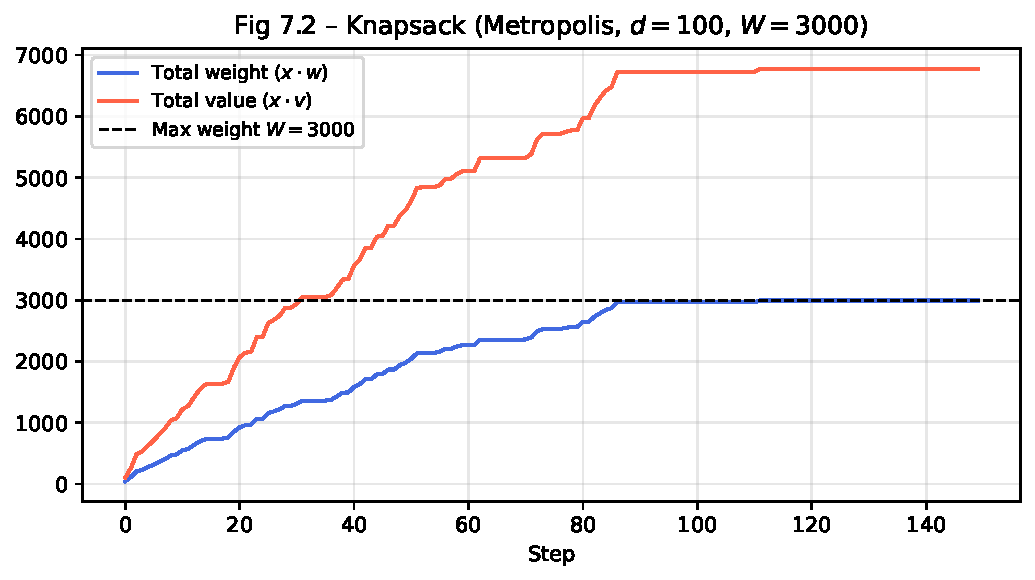
\includegraphics[width=\textwidth]{fig_knapsack_metropolis}
  \column{0.44\textwidth}
  \small
  The blue curve tracks total weight $\bx_k \cdot \bw$ and the red curve
  tracks total value $\bx_k \cdot \bv$.  Both rise rapidly as the knapsack
  fills, then level off as the algorithm refines its selection.\\[4pt]
  After 150 steps: total weight $\approx 2977$ (just below $W=3000$),
  total value $\approx 6745$.
\end{columns}

\begin{alertblock}{Key Insight}
  Both Gibbs and Metropolis naturally respect the capacity constraint by
  assigning zero probability to infeasible states --- no penalty term is
  needed.  The logistic conditional in Gibbs makes high-value items
  preferentially included, giving the chain a built-in greedy tendency at no
  extra algorithmic cost.
\end{alertblock}

\end{frame}

\begin{frame}[allowframebreaks]{The Boltzmann Distribution: Limiting Behaviour at Extreme Temperatures}

Before proceeding to individual algorithms, it is instructive to understand
concretely how the Boltzmann distribution $\pi^T_v \propto e^{-H(v)/T}$
(pi proportional to e to the negative H-of-v over T) behaves at extreme
temperatures through a numerical example.

\begin{exampleblock}{Worked Example: Three-State Space}
  Suppose $V = \{A, B, C\}$ with costs $H(A) = 1$, $H(B) = 3$, $H(C) = 7$.
  The Boltzmann weights at temperature $T$ are $e^{-1/T}$, $e^{-3/T}$,
  $e^{-7/T}$ respectively, and the normalising constant is
  $z_T = e^{-1/T} + e^{-3/T} + e^{-7/T}$.

  \medskip
  \begin{tabular}{lrrrl}
    \toprule
    Temperature $T$ & $\pi^T_A$ & $\pi^T_B$ & $\pi^T_C$ & Character\\
    \midrule
    $T = 10$ & 0.461 & 0.334 & 0.205 & Nearly uniform; free exploration\\
    $T = 1$  & 0.659 & 0.239 & 0.101 & $A$ clearly preferred\\
    $T = 0.5$& 0.841 & 0.113 & 0.046 & $A$ strongly preferred\\
    $T = 0.1$& 0.998 & 0.002 & $\approx 0$ & Essentially a point mass on $A$\\
    \bottomrule
  \end{tabular}

  \medskip
  State $A$ has the smallest cost $H(A) = 1$ and is the optimal solution.
  As $T \to 0$, $\pi^T_A \to 1$: the entire probability mass concentrates
  on the minimiser.  At high $T$, the distribution is spread out and the
  chain can explore freely.
\end{exampleblock}

\begin{alertblock}{The Fundamental Temperature Trade-off}
  Every algorithm in this chapter must choose a temperature (or a schedule
  of temperatures).  Too high: the chain explores freely but cannot reliably
  identify the optimum.  Too low: the optimum receives most probability but
  the chain mixes very slowly and gets stuck.  The five methods we study
  resolve this trade-off in different ways.
\end{alertblock}

\end{frame}

\begin{frame}[fragile]{Algorithm 61: Metropolis for Boltzmann Distribution}
  \begin{lstlisting}[style=python]
import numpy as np

def metropolis_boltzmann_step(v, neighbors, H, T, rng):
    """One Metropolis-Hastings step targeting Boltzmann pi^T (Alg. 61).
    v         : current state
    neighbors : dict mapping state -> list of neighbour states
    H         : cost function dict (H[v] = cost of state v)
    T         : temperature (float > 0)
    rng       : numpy RandomState
    """
    deg_v  = len(neighbors[v])
    v_prop = rng.choice(neighbors[v])          # propose uniformly random neighbour
    deg_vp = len(neighbors[v_prop])
    # Accept with min(1, deg(v)/deg(v') * exp((H(v)-H(v'))/T))
    alpha = min(1.0, (deg_v / deg_vp) * np.exp((H[v] - H[v_prop]) / T))
    return v_prop if rng.uniform() <= alpha else v

def run_metropolis(v0, neighbors, H, T, n_steps, seed=0):
    """Run Metropolis-Boltzmann for n_steps; return trajectory."""
    rng   = np.random.RandomState(seed)
    v     = v0
    chain = [v]
    for _ in range(n_steps):
        v = metropolis_boltzmann_step(v, neighbors, H, T, rng)
        chain.append(v)
    return chain
  \end{lstlisting}
\end{frame}

\begin{frame}[fragile]{Algorithms 63 \& 64: Gibbs and Metropolis for Knapsack}
  \begin{lstlisting}[style=python]
import numpy as np

def gibbs_knapsack_step(x, w, v, W, T, rng):
    """One Gibbs sampler step for 0-1 knapsack (Algorithm 63).
    x: current binary vector (length d), w,v: weight/value, W: capacity
    """
    d = len(x)
    i = rng.randint(0, d)                      # pick a random item
    weight_without_i = np.dot(w, x) - w[i] * x[i]
    if weight_without_i + w[i] > W:
        x[i] = 0                               # forced exclude: capacity exceeded
    else:
        # Conditional P(x_i=1) = 1/(1 + exp(-v_i/T)) -- logistic function
        prob1 = 1.0 / (1.0 + np.exp(-v[i] / T))
        x[i] = 1 if rng.rand() <= prob1 else 0
    return x

def metropolis_knapsack_step(x, w, v, W, T, rng):
    """One Metropolis step for 0-1 knapsack (Algorithm 64)."""
    d = len(x)
    i = rng.randint(0, d)
    x_new = x.copy()
    x_new[i] = 1 - x_new[i]                   # flip bit i
    if np.dot(w, x_new) <= W:                  # check feasibility
        # alpha=1 if adding item (x[i]=0), else exp(-v_i/T) if removing
        alpha = min(1.0, np.exp((1.0 / T) * (1 - 2 * x[i]) * v[i]))
        if rng.rand() < alpha:
            x[:] = x_new
    return x
  \end{lstlisting}
\end{frame}

% ============================================================
\section{7.2 Simulated Annealing}
% ============================================================

\begin{frame}[allowframebreaks]{7.2 Simulated Annealing: Motivation and Setup}

\textbf{The dilemma of fixed temperature.}
In the Metropolis algorithm at a fixed temperature $T$, there is a
fundamental trade-off between exploration and exploitation.  At
\textbf{high} $T$: the Boltzmann distribution $\pi^T$ is nearly uniform, so
the chain explores freely and escapes local minima easily --- but all states
have nearly equal probability, so the distribution puts little extra mass on
the global minimum and we cannot easily identify it from the chain's
trajectory.  At \textbf{low} $T$: $\pi^T$ is sharply concentrated near the
global minimum, which is exactly what we want --- but the chain mixes very
slowly because it gets trapped in local minima.  Any move to a higher-cost
state is accepted with probability $\approx e^{-\Delta H / T}$, which is
tiny for small $T$ and even modest energy barriers $\Delta H$.

Neither extreme works in isolation.  We need both exploration (to escape
local minima early on) and exploitation (to converge to the global minimum
eventually).

\medskip
\textbf{The Simulated Annealing solution.}
Simulated Annealing (SA) resolves this dilemma by starting at a high
temperature $T_0$ and gradually decreasing it according to a
\textbf{cooling schedule} $T_0 \ge T_1 \ge T_2 \ge \cdots \searrow 0$
(the symbol $\searrow$ means ``decreasing toward'').  The name ``annealing''
comes from metallurgy, where slowly cooling a heated metal allows atoms to
settle into a low-energy crystalline structure.  Rapid cooling (quenching)
produces a disordered, higher-energy structure; slow cooling produces a
near-optimal crystal.

At each step $k$, the chain uses the Metropolis transition probabilities
corresponding to temperature $T_k$.  This defines a
\emph{non-homogeneous} Markov chain: the transition matrix changes at every
step.

\begin{block}{SA Acceptance Probability at Step $k$}
  \[
    \alpha_k(v,v') = \min\!\left(1,\; e^{-(H(v')-H(v))/T_k}\right),
    \qquad v' \in \calN(v).
  \]
  \textbf{Notation:} $\alpha_k$ (alpha sub $k$) is the acceptance
  probability at step $k$.  $H(v') - H(v)$ is the cost increase if we move
  to $v'$ (positive means $v'$ is worse, negative means $v'$ is better).
  $T_k$ (T sub $k$) is the temperature at step $k$, which decreases
  over time.  When $T_k$ is large, $e^{-(H(v')-H(v))/T_k}$ is close to 1
  even for bad moves; when $T_k$ is small, only improvements are accepted.
\end{block}

\begin{alertblock}{How to Read the SA Acceptance Rule}
  A better move ($H(v') < H(v)$, so $H(v')-H(v) < 0$) is always accepted
  since the exponent is positive and $e^{\text{positive}} > 1$, so the
  minimum with 1 gives 1.  A worse move is accepted with probability
  $e^{-(H(v')-H(v))/T_k}$, which decreases as (i) the cost difference
  $H(v') - H(v)$ increases (more damage), or (ii) $T_k$ decreases (the
  algorithm becomes more selective).  This is the precise sense in which
  the algorithm becomes more conservative as it ``cools down''.
\end{alertblock}

\framebreak

\textbf{The modified Boltzmann distribution (Remark 7.2.1).}
When the graph $G$ is not regular (different states have different numbers
of neighbours), the stationary distribution of the Metropolis chain is the
\emph{modified} Boltzmann distribution:

\begin{block}{Modified Boltzmann Distribution (Eq.~7.2.1)}
  \[
    \pi^{T_k}_v = \frac{\deg(v)\exp(-H(v)/T_k)}{z_{T_k}}, \qquad v \in V,
  \]
  where $\deg(v)$ is the degree (number of neighbours) of $v$, and
  $z_{T_k} = \sum_{v'} \deg(v')\exp(-H(v')/T_k)$ is the normalising
  constant.  For regular graphs all $\deg(v)$ are equal, the factors cancel,
  and this reduces to the standard Boltzmann distribution.  Both
  distributions share the same minimiser of $H$, so the optimisation
  objective is unaffected.
\end{block}

\textbf{Proposition 7.2.2: concentrating mass on the optimum.}
Let $D^* = \{v \in V : H(v) = \min_{v'} H(v')\}$ be the set of optimal
solutions.  For any fixed temperature $T$, the chain (run at $T$ forever)
has stationary distribution $\pi^T$, and as $T \to 0$:
\[
  \sum_{v \in D^*} \pi^T_v \to 1.
\]
SA attempts to exploit this double limit by decreasing $T_k \to 0$
simultaneously with $k \to \infty$.

\framebreak

\textbf{How slow must the cooling be? Haj\'{e}k's condition.}
Suppose $v$ is a local minimum (not global).  Let
$c = \min_{v' \in \calN(v)} (H(v') - H(v)) > 0$ be the \textbf{energy
barrier} --- the smallest cost increase needed to escape from $v$.  The
probability of escaping $v$ in one step is at least $e^{-c/T_k}$ (since at
least one neighbour has cost increase $c$ and is accepted with that
probability).  For the chain to eventually escape $v$, the series of escape
probabilities must diverge:

\begin{block}{Cooling Schedule Requirement (Haj\'{e}k's Condition)}
  To guarantee eventual escape from every local minimum, the cooling
  schedule must satisfy:
  \[
    \sum_{k=0}^{\infty} e^{-c/T_k} = \infty.
  \]
  If this sum \emph{converges}, the chain can get permanently trapped in
  local minima with positive probability.  If it \emph{diverges}, the chain
  will eventually escape every local minimum.
\end{block}

The \textbf{logarithmic cooling schedule} $T_k = d / \log(k+2)$ (where $d$
is a constant at least as large as the energy barrier $c$) satisfies
Haj\'{e}k's condition because $e^{-c/T_k} = e^{-c\log(k+2)/d} = (k+2)^{-c/d}$
and the series $\sum_k (k+2)^{-c/d}$ diverges for $c/d \le 1$ (harmonic-like
series).  The \textbf{geometric cooling} $T_k = \beta^k T_0$ (where
$\beta$, pronounced ``bay-ta'', satisfies $0 < \beta < 1$) does \emph{not}
satisfy Haj\'{e}k's condition --- no global convergence guarantee.

\begin{exampleblock}{Checking Haj\'{e}k's Condition for Logarithmic Cooling}
  With $T_k = 1/\log(k+2)$ (setting $d=1$) and energy barrier $c=1$:
  \[
    e^{-c/T_k} = e^{-\log(k+2)} = \frac{1}{k+2}.
  \]
  Since $\sum_{k=0}^\infty 1/(k+2)$ is the harmonic series (which diverges),
  Haj\'{e}k's condition holds: SA with this schedule is guaranteed to find
  the global optimum.\\[4pt]
  With geometric cooling $T_k = 0.99^k$: $e^{-1/T_k} = e^{-1/0.99^k}$
  decreases to 0 super-exponentially fast, so $\sum_k e^{-1/T_k} < \infty$
  and there is no global guarantee.
\end{exampleblock}

\framebreak

\begin{columns}
  \column{0.54\textwidth}
  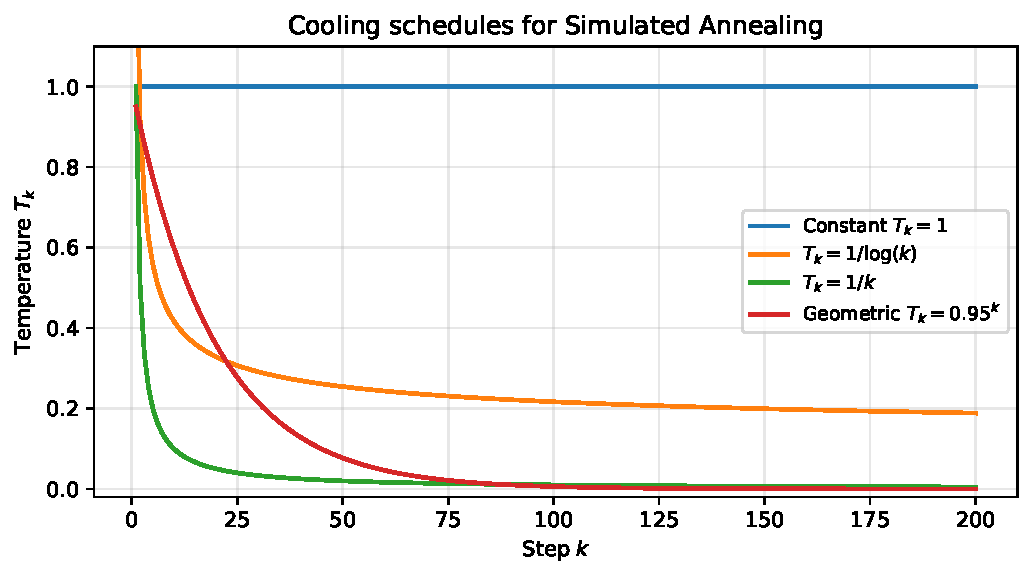
\includegraphics[width=\textwidth]{fig_cooling_schedule}
  \column{0.44\textwidth}
  \small
  \textbf{Common cooling schedules:}\\[4pt]
  \begin{itemize}
    \item \textbf{Constant} $T_k = T$: plain Metropolis; no convergence
      guarantee
    \item \textbf{Logarithmic} $T_k = d/\log(k+2)$: satisfies
      Haj\'{e}k's condition; guarantees global optimum; very slow in practice
    \item \textbf{Geometric} $T_k = \beta^k T_0$: popular in practice;
      fast; no global guarantee
    \item \textbf{Linear} $T_k = T_0(1-k/K)$: decreases too fast;
      usually fails
  \end{itemize}
  \vspace{4pt}
  The key requirement is that $T_k \searrow 0$ slowly enough that
  $\sum_k e^{-c/T_k} = \infty$.
\end{columns}

\end{frame}

\begin{frame}[allowframebreaks]{Non-Homogeneous Markov Chains and SA}

Because the transition matrix of SA changes at every step (the temperature
$T_k$ changes), it is not a standard (time-homogeneous) Markov chain and
requires the theory of \textbf{non-homogeneous Markov chains}.

\begin{block}{Definition: Time Non-Homogeneous Markov Chain}
  A sequence $(Y_n)$ is a \textbf{time non-homogeneous Markov chain}
  on a finite state space $\calS = \{s_1,\ldots,s_m\}$ if for any
  states $s_{i_0}, \ldots, s_{i_k} \in \calS$:
  \[
    \Prob(Y_0=s_{i_0}, Y_1=s_{i_1}, \ldots, Y_k=s_{i_k})
    = \mu_{s_{i_0}}\, p_{s_{i_0}s_{i_1}}(1)\,
      p_{s_{i_1}s_{i_2}}(2)\cdots p_{s_{i_{k-1}}s_{i_k}}(k),
  \]
  where $\mu$ (mu, pronounced ``myoo'') is the initial distribution and
  $p_{s_is_j}(k) = \Prob(Y_k = s_j \mid Y_{k-1} = s_i)$ is the
  \textbf{time-dependent} transition probability at step $k$.
\end{block}

\begin{block}{Distribution at Time $l$ (Eq.~7.2.3)}
  \[
    \bigl(\Prob(X_l=s_1), \ldots, \Prob(X_l=s_m)\bigr) = \bm{\mu}\,\mathbf{P}(0,l),
  \]
  where $\mathbf{P}(k,l) = \mathbf{P}(k)\mathbf{P}(k+1)\cdots\mathbf{P}(l)$
  is the product of transition matrices from step $k$ to step $l$.
  Each matrix $\mathbf{P}(k)$ has $(i,j)$ entry $p_{s_is_j}(k)$.  This
  is the non-homogeneous analogue of $\mu \mathbf{P}^l$ for a fixed matrix.
\end{block}

Simulated Annealing (Algorithm 65) is exactly a non-homogeneous Markov chain
with transition probabilities
$p_{vv'}(k) = q_{vv'}\alpha_k(v,v')$, where $q_{vv'}$ is the proposal
probability and $\alpha_k$ is the Metropolis acceptance probability at
temperature $T_k$.

\begin{columns}
  \column{0.54\textwidth}
  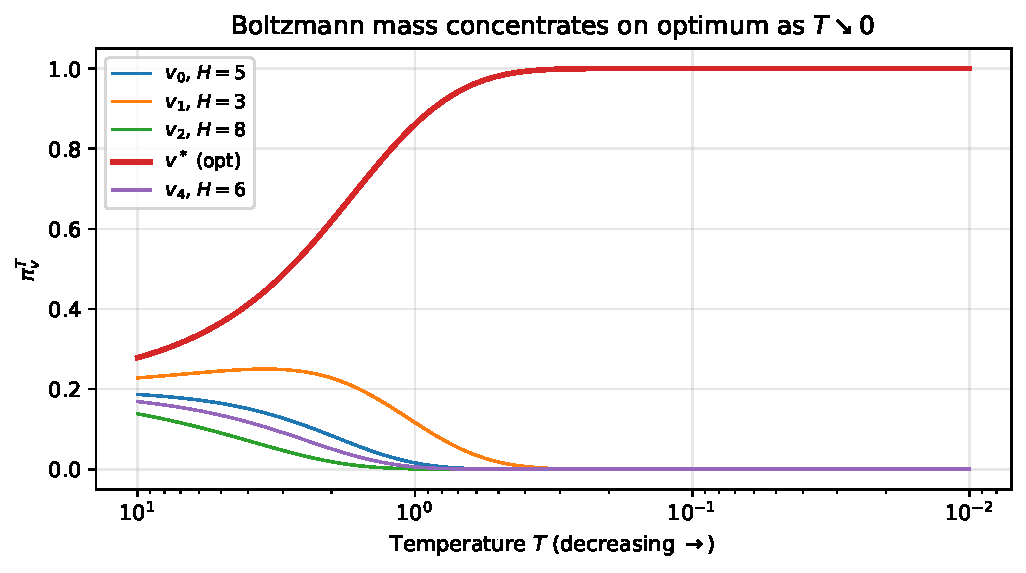
\includegraphics[width=\textwidth]{fig_nonhomogeneous_mc}
  \column{0.44\textwidth}
  \small
  As the temperature decreases along the cooling schedule, probability mass
  flows from high-cost states toward the optimal state(s).  With logarithmic
  cooling, $\Prob(X_k \in D^*) \to 1$ as $k \to \infty$.  The figure shows
  how the marginal distribution of the SA chain evolves over time.
\end{columns}

\end{frame}

\begin{frame}[fragile]{Algorithm 65: Simulated Annealing}
  \begin{lstlisting}[style=python]
import numpy as np

def sa_step(v, neighbors, H, T_k, rng):
    """One SA step at temperature T_k (Algorithm 65).
    v         : current state
    neighbors : adjacency dict, neighbors[v] = list of neighbours
    H         : cost function dict
    T_k       : current temperature (decreases over time)
    """
    v_prop  = rng.choice(neighbors[v])
    delta_H = H[v_prop] - H[v]
    # Accept improvements always; worse moves with exp(-delta_H/T_k)
    alpha_k = min(1.0, np.exp(-delta_H / T_k))
    return v_prop if rng.uniform() <= alpha_k else v

def simulated_annealing(v0, neighbors, H, cooling_schedule, n_steps, seed=0):
    """Run SA with a given cooling schedule. Returns trajectory + best.
    cooling_schedule: list [T_0, T_1, ...] or callable k -> T_k
    """
    rng    = np.random.RandomState(seed)
    v      = v0
    traj   = [v]
    best_v = v
    for k in range(n_steps):
        T_k = (cooling_schedule[k]
               if hasattr(cooling_schedule, '__getitem__')
               else cooling_schedule(k + 1))
        v = sa_step(v, neighbors, H, T_k, rng)
        traj.append(v)
        if H[v] < H[best_v]:
            best_v = v
    return traj, best_v

# Two standard cooling schedules:
def log_cooling(d=1.0):
    return lambda k: d / np.log(k + 2)        # T_k = d / log(k+2)

def geometric_cooling(T0=10.0, beta=0.99):
    return lambda k: T0 * beta**k              # T_k = T0 * beta^k
  \end{lstlisting}
\end{frame}

\begin{frame}[allowframebreaks]{7.2 SA for the Travelling Salesman Problem}

In the TSP the state space is $\calS = \mathcal{S}_n$ (all $n!$ tours of
$n$ cities).  We minimise the tour length $l(\sigma)$, which we cast as a
Boltzmann optimisation with $H(\sigma) = l(\sigma)$ and
$\pi^T_\sigma \propto e^{-l(\sigma)/T}$.

\medskip
\textbf{Proposal distribution: transpositions.}
Two tours $\sigma$ and $\sigma'$ are \emph{neighbours} if $\sigma'$ is
obtained from $\sigma$ by swapping exactly two city positions $i$ and $j$.
There are $\binom{n}{2}$ such transpositions, each proposed with
probability $q_{\sigma\sigma'} = 2/(n(n-1))$.  Since the graph is regular
(each tour has $\binom{n}{2}$ neighbours), the acceptance probability at
step $k$ simplifies to:
\[
  \alpha_k(\sigma,\sigma') = \min\!\left(1,\,e^{(l(\sigma)-l(\sigma'))/T_k}\right).
\]
If the proposed tour $\sigma'$ is shorter ($l(\sigma') < l(\sigma)$), then
$l(\sigma) - l(\sigma') > 0$ so $\alpha_k = 1$: shorter tours are always
accepted.  If the proposed tour is longer, the acceptance probability is
$e^{(l(\sigma)-l(\sigma'))/T_k} \in (0,1)$, which shrinks as $T_k$
decreases.

\begin{exampleblock}{Worked Example: One SA Step for TSP}
  Current tour: $\sigma = (1, 3, 2, 4)$, proposed swap of positions 2 and
  3: $\sigma' = (1, 2, 3, 4)$.  Suppose $\Delta l = l(\sigma') - l(\sigma)
  = +50$ miles (the proposed tour is 50 miles longer).  At $T_k = 100$:
  $\alpha = e^{-50/100} = e^{-0.5} \approx 0.607$: accept the worse tour
  with 60.7\% probability.  At $T_k = 10$: $\alpha = e^{-50/10} = e^{-5}
  \approx 0.007$: only 0.7\% acceptance.  As the temperature drops, the
  chain increasingly resists worsening moves, illustrating the cooling
  effect.
\end{exampleblock}

\textbf{2-opt variant (Remark 7.2.4).}
An often more effective proposal reverses a sub-segment of the tour.  Choose
indices $i < j$ uniformly at random and reverse the segment
$\sigma(i), \ldots, \sigma(j)$:
\[
  \sigma' = (\sigma(1),\ldots,\sigma(i-1),\,
            \underbrace{\sigma(j),\sigma(j-1),\ldots,\sigma(i)}_{\text{reversed}},\,
            \sigma(j+1),\ldots,\sigma(n)).
\]
This ``2-opt move'' is particularly effective because two edges that cross
in the plane are always replaced by non-crossing edges, typically reducing
tour length significantly.

\framebreak

\textbf{The 13-city USA benchmark.}

\begin{center}
  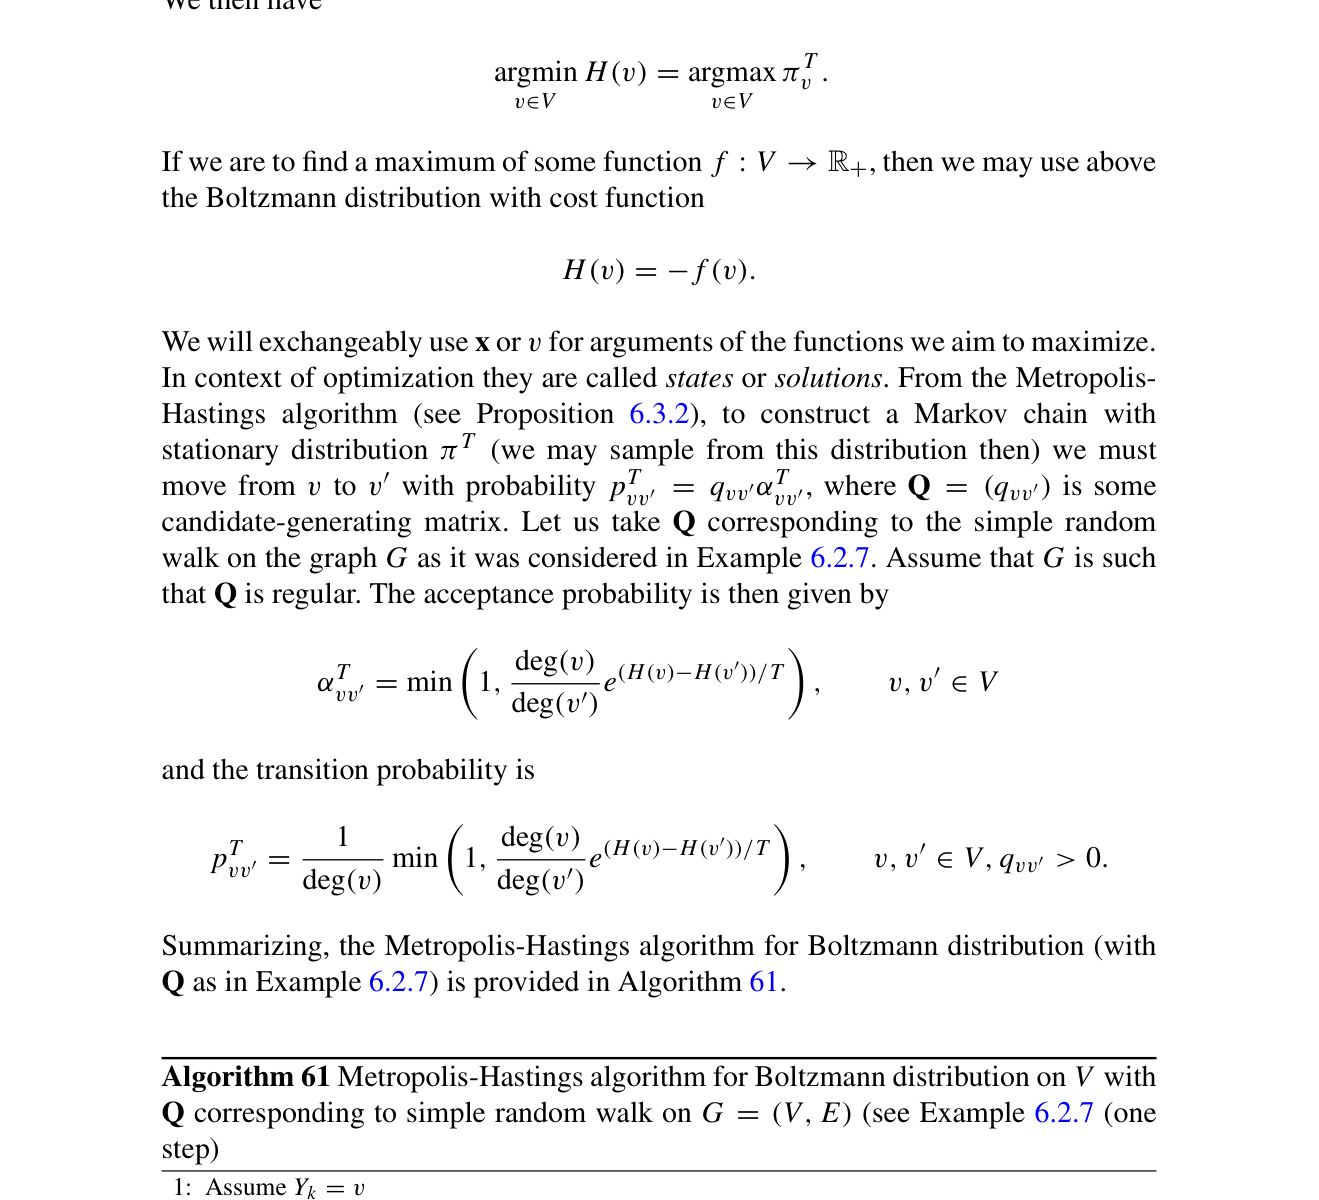
\includegraphics[width=0.70\textwidth]{fig_distance_matrix}
\end{center}

{\small \textbf{Figure: 13-city USA distance matrix.}
Entry $M(i,j) = M(j,i)$ is the road distance (in miles) between cities $i$
and $j$.  The diagonal $M(i,i) = 0$.  The optimal tour of length
\textbf{7024} was found by the Held--Karp dynamic-programming algorithm in
0.068 seconds.  A uniformly random tour has average length
$\approx 15938$ miles --- more than twice the optimal.}

\framebreak

\textbf{Benchmark results: Metropolis vs SA on 13-city TSP.}

\begin{center}
  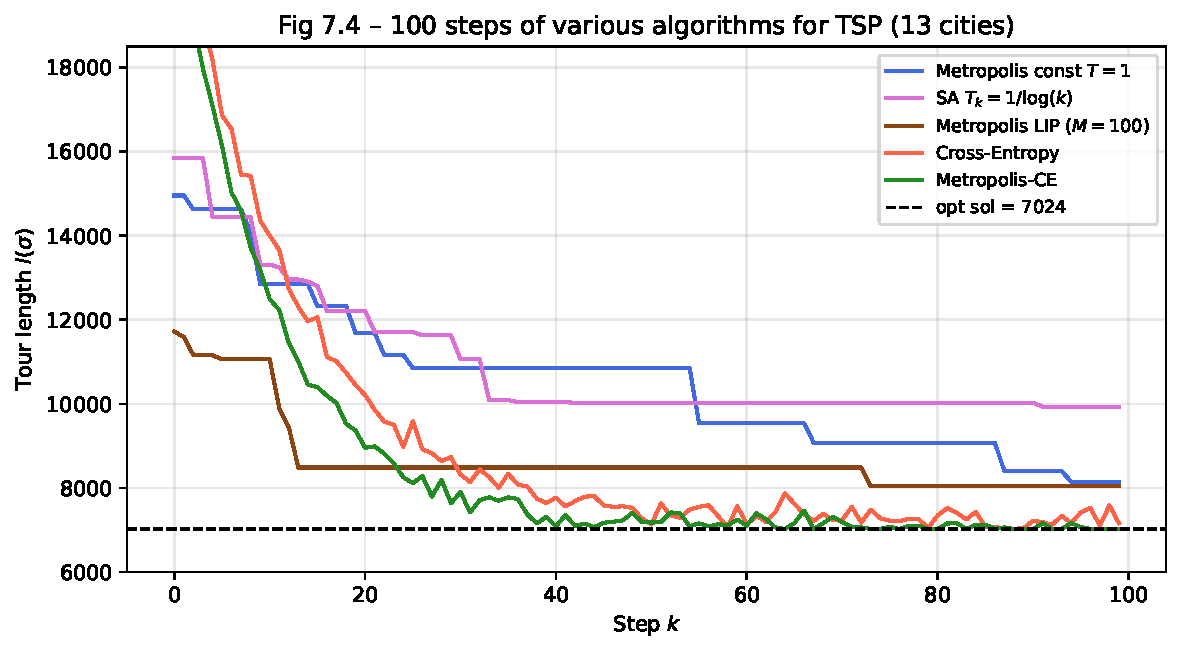
\includegraphics[width=0.68\textwidth]{fig_tsp_comparison}
\end{center}

{\small The dashed line at 7024 is the proven optimal tour length.  Running
both algorithms 100 times for 10 steps each, SA found better solutions in
approximately \textbf{60\%} of replications.  SA is advantageous early in
the run (when temperature is high) because it freely accepts worse moves and
escapes local minima.  As temperature drops, SA becomes increasingly
selective, gradually converging like Metropolis at low $T$.}

\begin{alertblock}{Key Takeaway: Simulated Annealing}
  SA improves on fixed-temperature Metropolis by combining free exploration
  (high $T$) with concentrated exploitation (low $T$).  With logarithmic
  cooling $T_k = d/\log(k+2)$, SA provably converges to the global optimum
  (Haj\'{e}k's theorem).  Geometric cooling ($T_k = \beta^k T_0$) is faster
  in practice but offers no such guarantee.
\end{alertblock}

\end{frame}

% ============================================================
\section{7.3 Locally Informed Proposals}
% ============================================================

\begin{frame}[allowframebreaks]{7.3 Locally Informed Proposals (LIP)}

\textbf{The limitation of uninformed Metropolis.}
In the standard Metropolis algorithm the proposal distribution $\mathbf{Q}$
is chosen independently of the target $\pi$ (pi): we propose a uniformly
random neighbour.  This is wasteful when many neighbours are clearly worse
than the current state.  For example, in the knapsack problem at a
near-optimal solution, most bit-flips that remove valuable items will be
rejected.  We waste proposal evaluations on moves we will not accept.

\medskip
\textbf{The LIP idea: let $\pi$ (pi) guide the proposal.}
Rather than choosing among all neighbours uniformly, we evaluate the
Boltzmann weight of each candidate neighbour and propose with probability
proportional to $g(\pi_{s'}/\pi_s)$, where $g : (0,\infty) \to (0,\infty)$
is a \emph{balancing function}.  This concentrates proposals on directions
where the target probability is higher.

Let $\calN(s) = \{s^{(1)},\ldots,s^{(M)}\}$ be a set of $M$ candidate
neighbours of the current state $s$ (sub-sampled from all neighbours).  The
\textbf{locally informed proposal distribution} is:

\begin{block}{LIP Distribution (Algorithm 68)}
  \[
    q^{\mathrm{LIP}}_{s, s^{(j)}}
    = \frac{1}{Z_g}\,g\!\left(\frac{\pi_{s^{(j)}}}{\pi_s}\right) q_{s, s^{(j)}},
    \qquad j = 1,\ldots,M.
  \]
  \textbf{Notation:} $q^{\mathrm{LIP}}_{s, s^{(j)}}$ (q-LIP from $s$ to
  $s^{(j)}$) is the informed proposal probability.
  $\pi_{s^{(j)}}/\pi_s$ is the ratio of target probabilities at the
  candidate neighbour versus the current state.
  $g(\pi_{s^{(j)}}/\pi_s)$ (g of the ratio) is the weight assigned to that
  neighbour --- larger when the neighbour is better.
  $q_{s,s^{(j)}}$ is the original uninformed proposal probability.
  $Z_g = \sum_{j=1}^{M} g(\pi_{s^{(j)}}/\pi_s)\, q_{s,s^{(j)}}$ is the
  normalising constant ensuring all proposal probabilities sum to 1.
\end{block}

The most common choice is $g(r) = \sqrt{r}$ (square root of $r$), which
satisfies the \emph{balancedness condition} $g(r) = r \cdot g(1/r)$.

\begin{alertblock}{How to Read the LIP Distribution}
  If a neighbour $s'$ has $\pi_{s'} \gg \pi_s$ (much better than current
  state), then $g(\pi_{s'}/\pi_s) = \sqrt{\pi_{s'}/\pi_s} \gg 1$, so $s'$
  is proposed far more often than under the uniform proposal.  The square
  root is a compromise: it strongly favours better neighbours but does not
  completely ignore worse ones, preventing degeneracy.  Think of it as a
  soft version of ``always go to the best neighbour''.
\end{alertblock}

\framebreak

\textbf{Metropolis--Hastings correction: why the acceptance ratio simplifies.}
Once a candidate $X$ is proposed from $q^{\mathrm{LIP}}_s$, the
Metropolis--Hastings acceptance probability corrects for the bias.  When the
balancing function satisfies $g(r) = r \cdot g(1/r)$ (as $\sqrt{r}$ does),
the acceptance probability simplifies to:

\begin{block}{LIP Acceptance Ratio with $g(r)=\sqrt{r}$}
  \[
    \alpha = \min\!\left(1,\; \frac{Z_g(s)}{Z_g(X)}\right).
  \]
  The acceptance probability depends only on the ratio of normalising
  constants at the current state $s$ and the proposed state $X$.
  $Z_g(s)$ and $Z_g(X)$ measure how ``rich'' (high-probability) the
  neighbourhoods of $s$ and $X$ are, respectively.
\end{block}

\begin{alertblock}{How to Read the LIP Acceptance Ratio}
  If the proposed state $X$ has a better-looking neighbourhood
  ($Z_g(X) > Z_g(s)$), then $Z_g(s)/Z_g(X) < 1$ and we accept with
  probability less than 1.  This balancing prevents the chain from being
  too greedy: it penalises moves to states with rich neighbourhoods, keeping
  the overall sampling distribution correct.  If $X$ has a worse-looking
  neighbourhood ($Z_g(X) < Z_g(s)$), we always accept (the ratio exceeds
  1, so the min gives 1).
\end{alertblock}

\begin{exampleblock}{Worked Example: LIP on a 3-Neighbour Graph}
  Suppose $\pi_A = 0.5$, $\pi_B = 0.3$, $\pi_C = 0.1$, $\pi_D = 0.1$,
  and $A$'s neighbours are $\{B, C, D\}$ with uniform $q = 1/3$.
  With $g(r) = \sqrt{r}$:
  \[
    Z_g(A) = \frac{1}{3}\bigl(\sqrt{0.3/0.5} + \sqrt{0.1/0.5} + \sqrt{0.1/0.5}\bigr)
    = \frac{1}{3}(0.775 + 0.447 + 0.447) = 0.556.
  \]
  The LIP proposal probabilities: $q^{\mathrm{LIP}}_{A,B} = 0.775/(3\times 0.556)
  = 0.465$ (46.5\%), while $q^{\mathrm{LIP}}_{A,C} = q^{\mathrm{LIP}}_{A,D}
  = 0.268$ (26.8\% each).  Under the uninformed proposal, $B$ would be
  proposed with only 33.3\%.  LIP has successfully biased the proposal
  toward the higher-probability neighbour $B$.
\end{exampleblock}

\framebreak

\textbf{Comparison on knapsack and TSP.}

\begin{columns}
  \column{0.50\textwidth}
  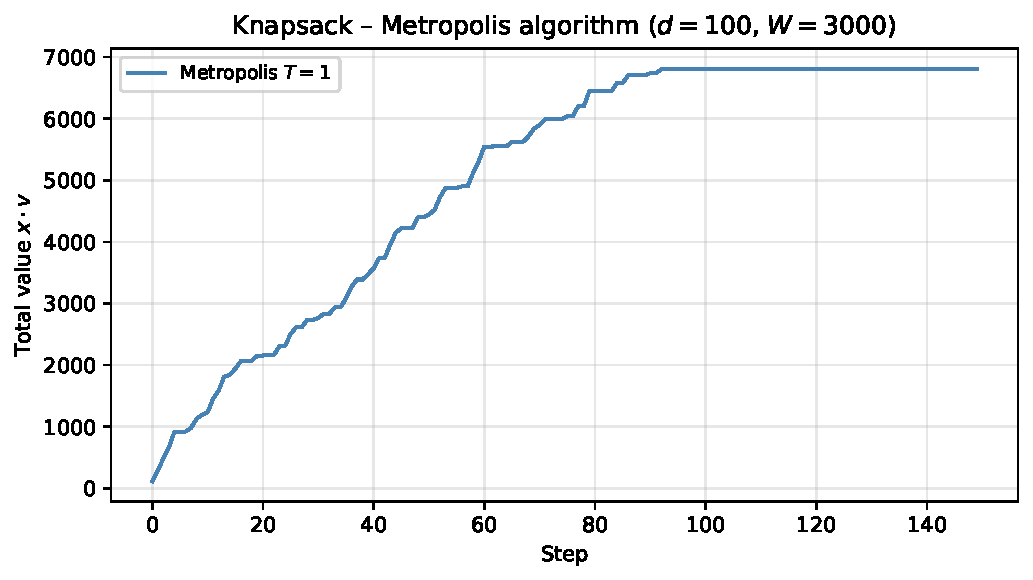
\includegraphics[width=\textwidth]{fig_lip_knapsack}
  \column{0.48\textwidth}
  \small
  \textbf{Knapsack ($d=100$, $M=100$ candidates):}\\
  LIP outperforms plain Metropolis because it preferentially proposes
  bit-flips that increase total value.  Nearly every step moves in a
  productive direction.\\[6pt]
  \textbf{TSP (13 cities, $M=100$ candidates):}\\
  In 100 replications, LIP won \textbf{9.66} times vs \textbf{0.33} for
  plain Metropolis --- LIP is approximately $29\times$ more likely to find
  the optimum per run.\\[4pt]
  \emph{Cost:} LIP requires evaluating $\pi$-ratios for $M$ neighbours per
  step versus 1 for plain Metropolis.  The quality improvement usually
  justifies this extra computation.
\end{columns}

\begin{alertblock}{Key Insight: LIP}
  LIP improves upon uninformed Metropolis by spending its ``proposal
  budget'' on the most promising directions while maintaining the exact
  stationary distribution $\pi^T$ via the Metropolis--Hastings correction.
  It is the discrete analogue of the Metropolis-Adjusted Langevin Algorithm
  (MALA), which uses the gradient to guide proposals in continuous spaces.
\end{alertblock}

\end{frame}

\begin{frame}[allowframebreaks]{LIP Acceptance Ratio: Full Derivation}

We now derive the Metropolis--Hastings acceptance ratio for LIP.
Recall the LIP proposal at current state $s$: propose state $s^{(j)}$ with
probability:
\[
  q^{\mathrm{LIP}}_{s,s^{(j)}} = \frac{g(\pi_{s^{(j)}}/\pi_s)\,q_{s,s^{(j)}}}{Z_g(s)},
  \qquad Z_g(s) = \sum_{l=1}^{M} g\!\left(\frac{\pi_{s^{(l)}}}{\pi_s}\right) q_{s,s^{(l)}}.
\]

Suppose the proposal selects $X = s^{(j)}$.  The Metropolis--Hastings
acceptance probability is:
\[
  \alpha = \min\!\left(1,\;
    \frac{\pi_X \cdot q^{\mathrm{LIP}}_{X,s}}{\pi_s \cdot q^{\mathrm{LIP}}_{s,X}}
  \right).
\]
The reverse proposal probability (from $X$, proposing $s$) is:
\[
  q^{\mathrm{LIP}}_{X,s} = \frac{g(\pi_s/\pi_X)\,q_{X,s}}{Z_g(X)}.
\]
Substituting and using symmetry $q_{X,s} = q_{s,X}$:
\[
  \frac{\pi_X\,q^{\mathrm{LIP}}_{X,s}}{\pi_s\,q^{\mathrm{LIP}}_{s,X}}
  = \frac{\pi_X \cdot g(\pi_s/\pi_X)}{\pi_s \cdot g(\pi_X/\pi_s)}
    \cdot \frac{Z_g(s)}{Z_g(X)}.
\]
When $g(r) = \sqrt{r}$: $g(\pi_s/\pi_X) = \sqrt{\pi_s/\pi_X}$ and
$g(\pi_X/\pi_s) = \sqrt{\pi_X/\pi_s}$, so:
\[
  \frac{\pi_X \cdot \sqrt{\pi_s/\pi_X}}{\pi_s \cdot \sqrt{\pi_X/\pi_s}}
  = \frac{\sqrt{\pi_X \pi_s}}{\sqrt{\pi_X \pi_s}} = 1.
\]
The first factor equals 1, leaving only the ratio of normalising constants:
$\alpha = \min(1,\, Z_g(s)/Z_g(X))$.

This beautiful simplification is the reason $g(r) = \sqrt{r}$ is the
standard choice.  Note that the Boltzmann weights $\pi_{s^{(j)}}$ need not
be computed absolutely --- only their ratios $\pi_{s^{(j)}}/\pi_s =
e^{(H(s)-H(s^{(j)}))/T}$ are needed, which are cheap to evaluate.

\textbf{LIP for TSP.}  In the TSP, the LIP weight for transposition $(i,j)$
producing tour $\sigma' = \tau_{ij}(\sigma)$ (sigma prime, the tour with
positions $i$ and $j$ swapped) is:
\[
  w_{ij} = g\!\left(\frac{\pi_{\sigma'}}{\pi_\sigma}\right)
  = e^{(l(\sigma)-l(\sigma'))/(2T)}.
\]
Transpositions that shorten the tour ($l(\sigma') < l(\sigma)$) get
$w_{ij} > 1$ (overweighted); tour-lengthening transpositions get
$w_{ij} < 1$ (underweighted).  The LIP proposal selects transposition
$(i,j)$ with probability proportional to $w_{ij}$.

\end{frame}

% ============================================================
\section{7.4 The Cross-Entropy Method}
% ============================================================

\begin{frame}[allowframebreaks]{7.4 The Cross-Entropy Method: Overview and Setup}

The Metropolis/SA/LIP methods are all \textbf{state-based}: they maintain a
single current solution and make small local moves.  The
\textbf{Cross-Entropy (CE) method} takes a fundamentally different approach:
it maintains a \emph{distribution over the entire solution space} and
iteratively shifts that distribution toward better solutions.

\medskip
\textbf{Setup.}
Let $h : \calS \to \R$ be the performance function to maximise.  Choose a
parametric family of distributions $\{p_{\btheta} : \btheta \in \Theta\}$
on $\calS$.  Here $\btheta$ (theta, pronounced ``thay-ta'') is the parameter
vector describing the distribution.  For example:
\begin{itemize}
  \item \textbf{Knapsack:} independent Bernoulli (Bernoulli means ``a
    coin flip'') coordinates,
    $p_{\btheta}(\bx) = \prod_{j=1}^d \theta_j^{x_j}(1-\theta_j)^{1-x_j}$,
    where $\theta_j \in [0,1]$ is the probability of including item $j$
    and $\btheta = (\theta_1,\ldots,\theta_d) \in [0,1]^d$.  The symbol
    $\prod_{j=1}^d$ (capital Pi, meaning ``product'') multiplies the
    Bernoulli factors for all $d$ items.
  \item \textbf{TSP:} a stochastic $n \times n$ matrix
    $\btheta = (\theta_{ij})$ with $\theta_{ii}=0$ and
    $\sum_j \theta_{ij} = 1$ for all $i$.  Here $\theta_{ij}$ is the
    probability of visiting city $j$ immediately after city $i$ in a
    sampled tour.
\end{itemize}

\begin{alertblock}{Comparing CE to Metropolis/SA/LIP}
  Metropolis tracks \emph{where we are} (a single solution); CE tracks
  \emph{what the best solutions look like} (a distribution).  CE is like
  learning a model of good solutions rather than navigating the landscape
  step by step.
\end{alertblock}

\framebreak

\textbf{Algorithm 69: The CE method for optimisation.}

The CE algorithm repeats the following two-step cycle until convergence:

\begin{enumerate}
  \item \textbf{Update the elite threshold $\gamma_t$ (gamma sub $t$).}
    Generate $M$ samples $X_1,\ldots,X_M \sim p_{\btheta'_{t-1}}$ from the
    current distribution.  Compute their performances $\eta_i = h(X_i)$ and
    sort them: $\eta_{(1)} \le \eta_{(2)} \le \cdots \le \eta_{(M)}$.  Set
    the elite threshold as the $(1-\rho)$-quantile (quantile, pronounced
    ``kwon-tile'', meaning the value below which a given fraction of the data
    falls):
    \[
      \gamma_t = \eta_{(\lceil(1-\rho)M\rceil)}.
    \]
    Here $\rho \in (0,1)$ (rho, pronounced ``roe'') is the \emph{elite
    fraction} (e.g., $\rho=0.1$ means the top 10\% are elite).  The notation
    $\lceil x \rceil$ means ``round $x$ up to the nearest integer''.

  \item \textbf{Update the parameter $\btheta'_t$.}
    Identify the elite set
    $\calE_t = \{X_i : h(X_i) \ge \gamma_t\}$ and solve the
    maximum-likelihood problem:
    \[
      \btheta' = \arg\max_{\btheta} \frac{1}{M}
        \sum_{i=1}^M \mathbf{1}(h(X_i)\ge\gamma_t)\log p_{\btheta}(X_i).
    \]
    This finds the parameter $\btheta$ that best explains the elite samples.
    Apply a \textbf{smoothed update} to prevent premature convergence:
    \[
      \btheta'_t = \alpha\,\btheta' + (1-\alpha)\,\btheta'_{t-1}.
    \]
    Here $\alpha \in (0,1)$ (alpha) is the smoothing parameter (typically
    $\alpha = 0.7$): larger $\alpha$ adapts faster; smaller $\alpha$ is
    more stable.
\end{enumerate}

\textbf{Stopping criterion:} terminate when the elite threshold $\gamma_t$
has not improved for $d$ consecutive iterations (default $d=5$).

\begin{center}
  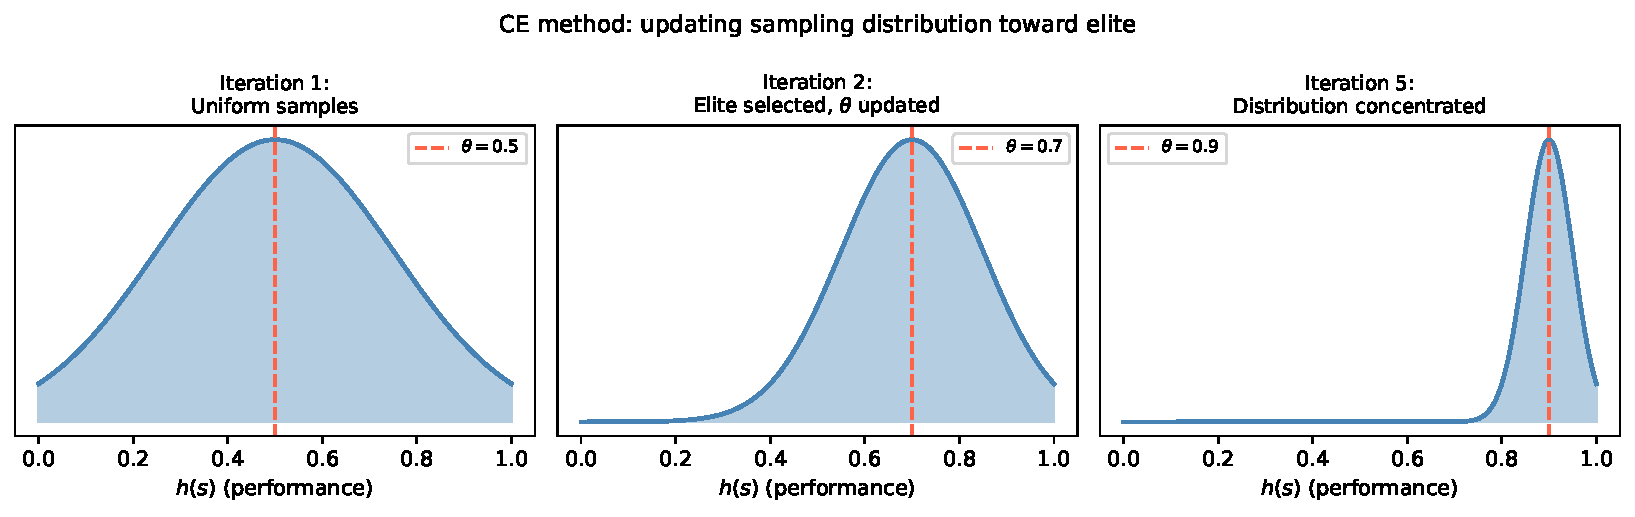
\includegraphics[width=0.80\textwidth]{fig_ce_schematic}
\end{center}
{\small At each iteration $t$, the distribution $p_{\btheta'_{t-1}}$ is
sampled, the top $\rho$-fraction by performance forms the elite set
(shaded), and the new parameter $\btheta'_t$ is fitted to the elites.  The
distribution shifts toward the high-performance region with each iteration.}

\end{frame}

\begin{frame}[allowframebreaks]{CE for the Knapsack: Closed-Form Update Derivation}

For the knapsack the parametric family is independent Bernoullis:
$p_{\btheta}(\bx) = \prod_{j=1}^d \theta_j^{x_j}(1-\theta_j)^{1-x_j}$.
Taking the logarithm (to convert the product into a sum):
\[
  \log p_{\btheta}(\bx) = \sum_{j=1}^d
  \bigl[x_j \log\theta_j + (1-x_j)\log(1-\theta_j)\bigr].
\]

To find $\btheta'$, we differentiate the CE objective with respect to
$\theta_k$ (theta sub $k$, the probability of including item $k$) and set
the derivative to zero:
\begin{align*}
  0 &= \frac{\partial}{\partial\theta_k}
    \frac{1}{M}\sum_{i=1}^M \mathbf{1}(h(X_i)\ge\gamma_t)\log p_{\btheta}(X_i)
  = \frac{1}{M\theta_k(1-\theta_k)}\sum_{i=1}^M
    \mathbf{1}(h(X_i)\ge\gamma_t)(X_i(k) - \theta_k).
\end{align*}
Solving for $\theta_k$ yields a beautifully simple result:

\begin{block}{CE Update for Knapsack (Eq.~7.4.7)}
  \[
    \theta'_k = \frac{\displaystyle\sum_{i=1}^M
      \mathbf{1}(h(X_i)\ge\gamma_t)\,X_i(k)}
             {\displaystyle\sum_{i=1}^M \mathbf{1}(h(X_i)\ge\gamma_t)}
    = \text{fraction of elite samples that include item } k.
  \]
  \textbf{Notation:} $X_i(k) \in \{0,1\}$ is the $k$-th coordinate of
  sample $X_i$ (is item $k$ selected in solution $i$?).  The indicator
  $\mathbf{1}(h(X_i)\ge\gamma_t)$ equals 1 if sample $i$ is elite and 0
  otherwise.  The formula computes the fraction of elite samples that have
  item $k$ selected.
\end{block}

\begin{alertblock}{How to Read the CE Knapsack Update}
  This is simply the sample mean of the elite samples' $k$-th coordinates.
  If item $k$ appears in 80\% of the elite solutions, then $\theta'_k = 0.8$:
  the next iteration will include item $k$ with 80\% probability.  Over
  iterations: $\theta_k \to 1$ for items always in elite solutions (the
  algorithm decides to always include them) and $\theta_k \to 0$ for items
  never in elite solutions.  The CE method is therefore learning a
  probabilistic model of what good solutions look like.
\end{alertblock}

\begin{exampleblock}{Worked Example: 3-Item Knapsack CE Update}
  Suppose $d = 3$, $M = 5$ samples, elite fraction $\rho = 0.4$
  (top 40\%, so 2 out of 5 samples are elite).  The 2 elite solutions are:
  $\bx^{(1)} = (1,1,0)$ (items 1 and 2 selected) and
  $\bx^{(2)} = (1,0,1)$ (items 1 and 3 selected).  The CE update gives:
  \[
    \theta'_1 = \frac{1+1}{2} = 1.0, \quad
    \theta'_2 = \frac{1+0}{2} = 0.5, \quad
    \theta'_3 = \frac{0+1}{2} = 0.5.
  \]
  Item 1 appears in both elite solutions so $\theta'_1 = 1.0$.  After
  smoothing with $\alpha=0.7$ and prior $\btheta = (0.5, 0.5, 0.5)$:
  \[
    \btheta'_t = 0.7 \cdot (1, 0.5, 0.5) + 0.3 \cdot (0.5, 0.5, 0.5)
    = (0.85, 0.5, 0.5).
  \]
  Without smoothing, $\theta'_1$ would jump to 1 immediately and stay there,
  which could be premature if the sample was unlucky.
\end{exampleblock}

\framebreak

\textbf{Convergence of the CE method for the knapsack.}

\begin{center}
  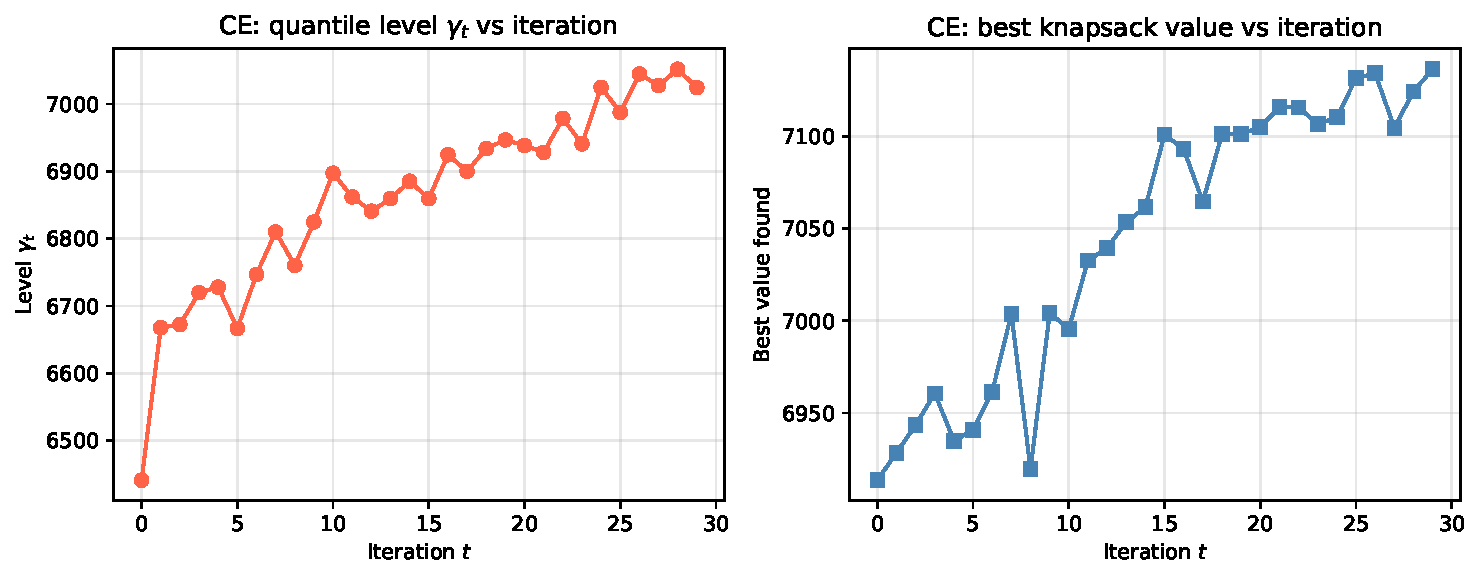
\includegraphics[width=0.76\textwidth]{fig_ce_convergence}
\end{center}
{\small \textbf{Left panel:} the elite quantile $\gamma_t$ (gamma sub $t$)
increases monotonically over CE iterations, tracking the improvement in
solution quality.  \textbf{Right panel:} the best value found in each batch
improves rapidly and then plateaus.  CE typically converges in approximately
30 iterations for $d=100$, each using $M=200$ samples.}

\framebreak

\begin{columns}
  \column{0.50\textwidth}
  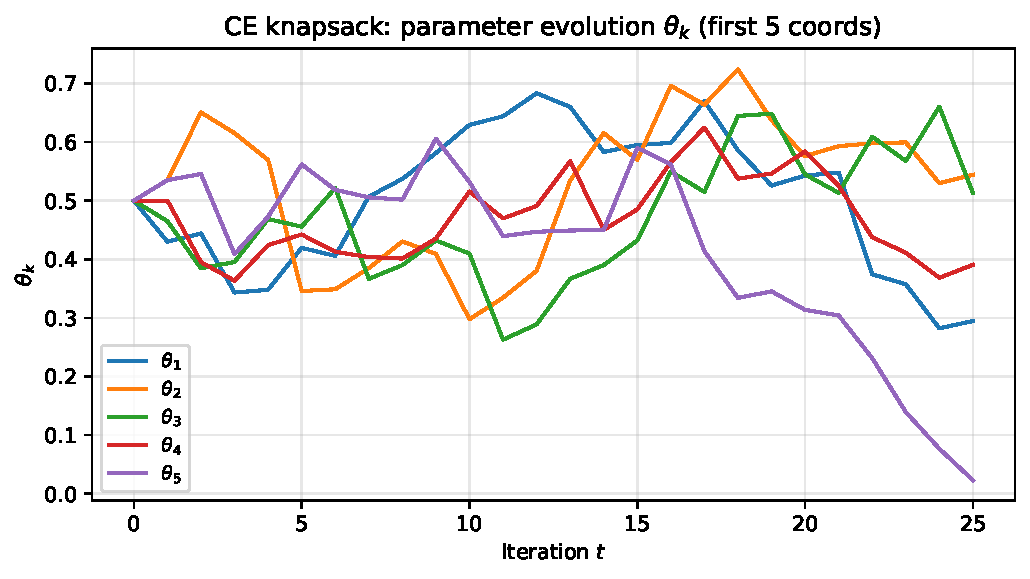
\includegraphics[width=\textwidth]{fig_ce_theta}
  \column{0.48\textwidth}
  \small
  \textbf{Evolution of $\theta_k$ (theta sub $k$) parameters over CE iterations.}\\[4pt]
  Each curve represents one coordinate $\theta_k$ --- the probability that
  item $k$ is included in a sampled solution.  Over iterations:
  \begin{itemize}
    \item $\theta_k \to 1$: item $k$ appears in every elite solution ---
      the algorithm decides to always include it.
    \item $\theta_k \to 0$: item $k$ never appears in elite solutions ---
      the algorithm decides to never include it.
  \end{itemize}
  Items with the highest value-to-weight ratio $v_i/w_i$ converge to 1
  first.  Smoothing (with $\alpha=0.7$) prevents premature convergence.
\end{columns}

\end{frame}

\begin{frame}[fragile]{CE for the Knapsack: Python Implementation}
  \begin{lstlisting}[style=python,basicstyle=\ttfamily\tiny]
import numpy as np

def ce_knapsack(d, w, v, W, theta0, M=200, rho=0.1, alpha=0.7,
                d_stop=5, max_iter=50):
    """Cross-Entropy method for 0-1 Knapsack (Algorithm 69).
    d: num items;  w,v: weight/value arrays;  W: capacity
    theta0: initial Bernoulli params (shape d, e.g. all 0.5)
    M: sample size;  rho: elite fraction;  alpha: smoothing param
    """
    theta = theta0.copy()
    best_val, gamma_history = [], []
    for t in range(max_iter):
        # Step 1: sample M binary vectors from independent Bernoulli(theta)
        X = (np.random.rand(M, d) < theta).astype(float)
        # Compute performances (0 for infeasible solutions)
        h_vals = np.array([x @ v if x @ w <= W else 0.0 for x in X])
        # Step 2: compute (1-rho)-quantile = elite threshold gamma_t
        gamma_t = np.quantile(h_vals, 1 - rho)
        gamma_history.append(gamma_t)
        # Step 3: theta' = fraction of elite samples with x_k=1 (Eq. 7.4.7)
        elite_mask = h_vals >= gamma_t
        if elite_mask.sum() > 0:
            theta_new = X[elite_mask].mean(axis=0)
            theta = alpha * theta_new + (1 - alpha) * theta  # smoothed update
        best_val.append(h_vals.max())
        # Stop if elite level unchanged for d_stop consecutive iterations
        if (len(gamma_history) > d_stop and
                len(set(round(g, 6) for g in gamma_history[-d_stop:])) == 1):
            break
    return theta, best_val, gamma_history
  \end{lstlisting}
\end{frame}

\begin{frame}[allowframebreaks]{CE for the TSP: Stochastic-Matrix Parametrisation}

For the TSP, we need a parametric family over permutations of $n$ cities.
The natural choice is a stochastic $n \times n$ matrix
$\btheta = (\theta_{ij})$ with $\theta_{ii} = 0$ and $\sum_j \theta_{ij} = 1$
for all $i$.  Here $\theta_{ij}$ (theta sub $ij$) is the probability that
city $j$ is visited immediately after city $i$ in a sampled tour.

Over iterations, as CE learns from elite tours: $\theta_{ij} \to 1$ for
edges $(i \to j)$ that appear in the best tours and $\theta_{ij} \to 0$ for
edges that never appear.

\begin{block}{Algorithm 70: Sampling a Tour from $\btheta$}
  Fix the starting city as $\sigma_1 = 1$.  For $k = 1, \ldots, n-1$:
  \begin{enumerate}
    \item Take row $\sigma_k$ of $\btheta$: $\mathbf{r}^{k+1} = \btheta(\sigma_k, \cdot)$.
    \item Zero out entries for already-visited cities:
      set $r^{k+1}_j = 0$ for all $j$ already visited.
    \item Normalise the remaining entries: $q^{k+1}_j = r^{k+1}_j / \sum_i r^{k+1}_i$.
    \item Sample the next city: $\sigma_{k+1} \sim \mathbf{q}^{k+1}$.
  \end{enumerate}
  This greedy sequential sampling produces a valid tour (no repeated cities)
  because we zero out visited cities before sampling.
\end{block}

\begin{block}{CE Update for TSP (Eq.~7.4.9)}
  \[
    \theta'_{ab}
    = \frac{\displaystyle\sum_{i=1}^M \mathbf{1}(h(X_i)\ge\gamma_t)
             \sum_{k=1}^{n-1}\mathbf{1}(\sigma_k^{(i)}=a,\,\sigma_{k+1}^{(i)}=b)}
           {\displaystyle\sum_{b'=1}^n \sum_{i=1}^M \mathbf{1}(h(X_i)\ge\gamma_t)
             \sum_{k=1}^{n-1}\mathbf{1}(\sigma_k^{(i)}=a,\,\sigma_{k+1}^{(i)}=b')}.
  \]
  \textbf{Notation:} $\theta'_{ab}$ (theta-prime sub $ab$) is the updated
  probability of going from city $a$ to city $b$.  The numerator counts how
  many times the directed edge $a \to b$ appears in elite tours.  The
  denominator counts how many times \emph{any} edge leaving city $a$ appears
  in elite tours.  The ratio is row-normalised so each row of $\btheta'$
  sums to 1.
\end{block}

\begin{alertblock}{How to Read the TSP CE Update}
  If city $j$ frequently follows city $i$ in the best tours found so far,
  then $\theta'_{ij}$ is large and the next round of sampling will also tend
  to visit $j$ after $i$.  Over iterations, the matrix $\btheta$ converges
  to (approximately) the permutation matrix of the optimal tour: a matrix
  with exactly one 1 in each row (the optimal next city) and zeros
  elsewhere.
\end{alertblock}

\begin{exampleblock}{Convergence intuition for a 4-city TSP}
  Suppose the optimal tour is $1 \to 3 \to 2 \to 4 \to 1$.  Then over
  iterations: $\theta_{13} \to 1$, $\theta_{32} \to 1$, $\theta_{24} \to 1$,
  $\theta_{41} \to 1$, while all other entries $\to 0$.  Sampling from this
  converged $\btheta$ almost certainly produces the optimal tour every time.
\end{exampleblock}

\end{frame}

\begin{frame}[fragile]{CE for TSP: Python Implementation}
  \begin{lstlisting}[style=python,basicstyle=\ttfamily\tiny]
import numpy as np

def sample_tour(theta, n, rng):
    """Algorithm 70: sample a tour from stochastic matrix theta."""
    sigma = [0]          # always start at city 0 (0-indexed)
    for k in range(n - 1):
        row = theta[sigma[-1]].copy()
        for already in sigma:
            row[already] = 0.0     # exclude already-visited cities
        row /= row.sum()           # normalise remaining probabilities
        sigma.append(rng.choice(n, p=row))
    return sigma

def tour_length(sigma, M_dist):
    """Total tour length for permutation sigma and distance matrix."""
    n = len(sigma)
    return (sum(M_dist[sigma[k], sigma[k+1]] for k in range(n-1))
            + M_dist[sigma[-1], sigma[0]])

def ce_tsp_update(elite_tours, n, alpha=0.7, theta_prev=None):
    """Compute theta' from elite tours via Eq. 7.4.9, with smoothing."""
    counts = np.zeros((n, n))
    for tour in elite_tours:
        for k in range(len(tour) - 1):
            counts[tour[k], tour[k + 1]] += 1  # count directed edge a->b
    row_sums = counts.sum(axis=1, keepdims=True)
    row_sums[row_sums == 0] = 1.0   # avoid division by zero
    theta_new = counts / row_sums   # row-normalise: each row sums to 1
    if theta_prev is not None:
        theta_new = alpha * theta_new + (1 - alpha) * theta_prev
    return theta_new
  \end{lstlisting}
\end{frame}

% ============================================================
\section{7.5 The Metropolis Cross-Entropy Hybrid}
% ============================================================

\begin{frame}[allowframebreaks]{7.5 The Metropolis Cross-Entropy: A Hybrid Approach}

\textbf{Comparing the two paradigms.}
Metropolis-based algorithms maintain a \emph{single current solution}
$X^{(t)}$ and make small local moves guided by the target distribution.  At
each step, one new solution is evaluated.  The CE method maintains a
\emph{distribution parameter} $\btheta'_{t-1}$ over the \emph{entire}
solution space and generates $M$ independent samples at each step.  The
state is a parameter, not a solution.

\medskip
\textbf{The Metropolis-CE hybrid idea (Algorithm 72).}
The Metropolis-CE algorithm combines both paradigms.  At each step $t$:
\begin{enumerate}
  \item Generate $M$ neighbours of the current solution $X^{(t-1)}$ by
    sampling from the \emph{adaptive transition distribution}
    $Q_{\btheta'_{t-1}}(X^{(t-1)}, \cdot)$.
  \item Compute the elite threshold $\gamma_t$ (gamma sub $t$) from these
    $M$ neighbours' performances.
  \item Update $\btheta'_t$ via CE maximum-likelihood on the elite
    neighbours.
  \item Set $X^{(t)}$ to the best-performing neighbour found.
\end{enumerate}

The key difference from plain CE: rather than sampling $M$ solutions from
the global distribution over $\calS$, we sample $M$ \emph{neighbours} of
the current solution.  The parameter $\btheta$ controls which types of local
moves to prefer --- and it adapts based on which moves have been elite.

\begin{block}{Metropolis-CE Parameter Update (Eq.~7.5.1)}
  \[
    \btheta' = \arg\max_{\btheta} \frac{1}{M}
      \sum_{i=1}^M \mathbf{1}(h(X_i) \ge \gamma_t)
      \log Q_{\btheta}(X^{(t-1)}, X_i).
  \]
  \textbf{Notation:} $Q_{\btheta}(X^{(t-1)}, X_i)$ is the transition
  probability from the current state $X^{(t-1)}$ to neighbour $X_i$ under
  parameter $\btheta$.  The likelihood focuses learning on which moves from
  the current position are most productive.
\end{block}

\framebreak

\textbf{Metropolis-CE for the Knapsack: derivation.}
From the current state $\bx = X^{(t-1)}$, flip coordinate $k$ with
probability $\theta_k \ge 0$, where $\sum_k \theta_k = 1$ (so
$\boldsymbol{\theta}$ is a probability distribution over the $d$ possible
bit-flips).  A neighbour $X_i$ produced by flipping coordinate $a_i$
contributes $\log Q_{\boldsymbol{\theta}}(X^{(t-1)}, X_i) = \log \theta_{a_i}$.

The CE objective with constraint $\sum_k \theta_k = 1$ is maximised via
Lagrange multipliers (lambda, $\lambda$, a method for constrained
optimisation):
\[
  \mathcal{L}(\boldsymbol{\theta}, \lambda) = \frac{1}{M}\sum_{i=1}^M
  \mathbf{1}(h(X_i) \ge \gamma_t)\log \theta_{a_i}
  + \lambda\!\left(1 - \sum_{k=1}^d \theta_k\right).
\]
Setting $\partial\mathcal{L}/\partial\theta_k = 0$ and solving yields:

\begin{block}{CE Update for Knapsack Transitions}
  \[
    \theta'_k = \frac{C_k}{\sum_{j=1}^d C_j},
    \quad
    C_k = \#\{\text{elite samples in which coordinate }k\text{ was flipped}\}.
  \]
  Here $C_k$ (C sub $k$) counts how often flipping bit $k$ produced an
  elite neighbour.  The update $\theta'_k$ is large if bit-flip $k$
  frequently leads to elite neighbours from the current state.
\end{block}

\begin{alertblock}{How to Read the Metropolis-CE Update}
  The algorithm is learning \emph{which moves from the current position are
  most productive}.  If bit 73 has been frequently responsible for elite
  improvements in recent steps, $\theta_{73}$ grows large and future steps
  will try flipping bit 73 more often.  This is local adaptive learning,
  unlike CE which learns global structure.
\end{alertblock}

Running with $\rho=0.3$, $M=30$, $\alpha=0.001$ for 100 steps:
Metropolis-CE won \textbf{100 out of 100} replications on the knapsack.

\framebreak

\textbf{Metropolis-CE for the TSP.}
For the TSP, the parameter $\boldsymbol{\theta} = (\theta(i,j))_{i<j}$ is a
probability distribution over all $n(n-1)/2$ possible transpositions (swaps
of positions $i$ and $j$), satisfying $\sum_{i<j}\theta(i,j) = 1$.  The CE
update is:

\begin{block}{CE Update for TSP Swaps (Eq.~7.5.2)}
  \[
    \theta'(a,b)
    = \frac{C_{(a,b)}}{\displaystyle\sum_{i<j} C_{(i,j)}},
    \quad
    C_{(a,b)} = \#\{\text{elite samples using swap }(a,b)\}.
  \]
  The weight $\theta'(a,b)$ grows large when swapping positions $a$ and $b$
  frequently produces elite solutions, so future proposals preferentially
  try swaps that have been historically productive.
\end{block}

\begin{center}
  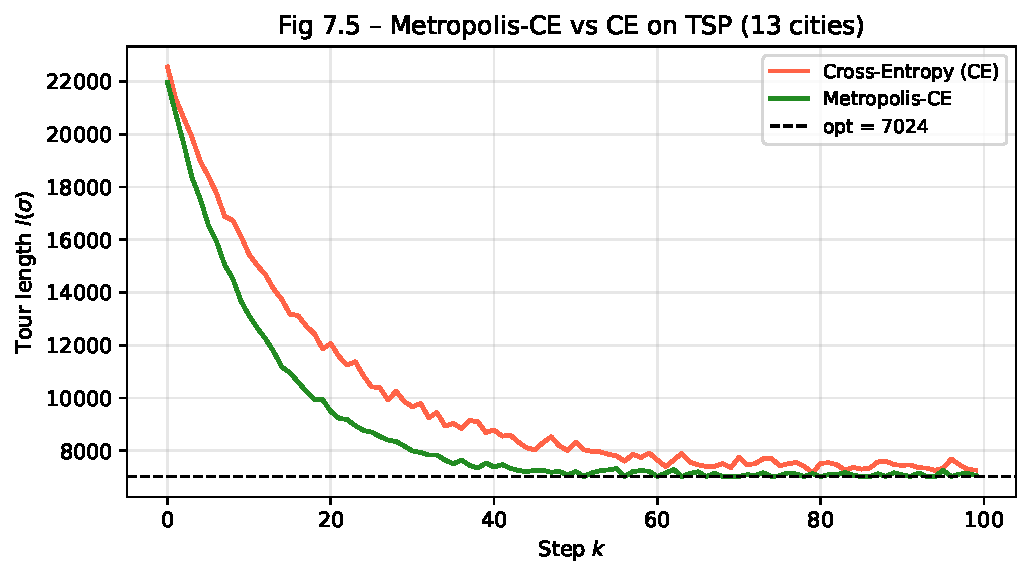
\includegraphics[width=0.43\textwidth]{fig_mce_vs_ce}
\end{center}

\begin{block}{TSP Win Scores (100 replications, 100 steps each)}
  CE: 61 wins; Metropolis-CE: 29 wins; LIP: 9.66 wins; plain Metropolis:
  0.33 wins.  Metropolis-CE achieves comparable quality to CE at roughly
  $23\times$ lower computational cost.
\end{block}

\end{frame}

\begin{frame}[fragile]{Algorithm 72: Metropolis-CE Hybrid (Python)}
  \begin{lstlisting}[style=python]
import numpy as np

def metropolis_ce_knapsack(x0, w, v, W, T=100, M=30, rho=0.3, alpha=0.001):
    """Metropolis-CE hybrid for 0-1 knapsack (Algorithm 72).
    x0: initial binary vector (length d)
    theta: probability vector over d bit-flips (which bit to flip)
    """
    d = len(x0)
    x_cur  = x0.copy()
    theta  = np.ones(d) / d          # initially uniform over all bit-flips
    best_x = x_cur.copy()
    best_h = x_cur @ v if x_cur @ w <= W else 0.0

    for t in range(1, T + 1):
        # Step 1: generate M neighbours by flipping bits according to theta
        flip_bits = np.random.choice(d, size=M, p=theta)
        neighbors = []
        for k_flip in flip_bits:
            nb = x_cur.copy()
            nb[k_flip] = 1 - nb[k_flip]   # flip bit k_flip
            neighbors.append((k_flip, nb))
        perfs = np.array([nb @ v if nb @ w <= W else 0.0
                          for (_, nb) in neighbors])
        # Step 2: elite threshold (top rho fraction)
        gamma_t    = np.quantile(perfs, 1 - rho)
        elite_mask = perfs >= gamma_t
        # Step 3: CE update -- count how often each bit-flip is elite
        if elite_mask.sum() > 0:
            C = np.zeros(d)
            for idx in np.where(elite_mask)[0]:
                C[neighbors[idx][0]] += 1
            if C.sum() > 0:
                theta_new = C / C.sum()
                theta = alpha * theta_new + (1 - alpha) * theta
        # Step 4: move to best-performing neighbour
        best_idx = int(np.argmax(perfs))
        x_cur = neighbors[best_idx][1].copy()
        if perfs[best_idx] > best_h and x_cur @ w <= W:
            best_x = x_cur.copy()
            best_h = perfs[best_idx]
    return best_x, best_h
  \end{lstlisting}
\end{frame}

% ============================================================
\section{7.6 Summary of Simulation Results}
% ============================================================

\begin{frame}[allowframebreaks]{7.6 Summary of Simulation Results}

\textbf{Experimental setup.}
All five algorithms were run on \textbf{100 replications} of each benchmark.
For each replication the algorithm ran for a fixed number of steps and we
recorded the best solution found.  A ``win'' means the algorithm found the
strictly best solution among all five algorithms run with the same random
seed.  Win fractions sum to 100 (ties split equally).

\textbf{7.6.1 Travelling Salesman Problem (13 cities)}

The 13-city USA instance has optimal tour length \textbf{7024 miles}
(Held--Karp, 0.068 s).  A uniformly random tour has average length
$\approx 15938$ miles.

\begin{center}
  \small
  \begin{tabular}{lrrl}
    \toprule
    Algorithm & Win score & Approx.\ best & Runtime\\
    \midrule
    Metropolis ($T=1$, constant)         & 0.33  & $\sim 9000$ miles  & $< 1$\,s\\
    Simulated Annealing ($T_k=1/\log k$) & 0.00  & $\sim 8000$ miles  & $< 1$\,s\\
    LIP ($M=100$ candidates)             & 9.66  & $\sim 7500$ miles  & $\sim 10$\,s\\
    Cross-Entropy (Alg.~71)              & 61.0  & $\sim 7300$ miles  & $\sim 230$\,s\\
    Metropolis-CE (Alg.~72)              & 29.0  & $\sim 7050$ miles  & $\sim 10$\,s\\
    \midrule
    Held--Karp (exact)                   & ---   & \textbf{7024} miles & 0.068\,s\\
    \bottomrule
  \end{tabular}
\end{center}

\small
Win scores are averages over 100 replications; they do not sum to exactly
100 because of fractional tie-splitting.

\framebreak

\begin{center}
  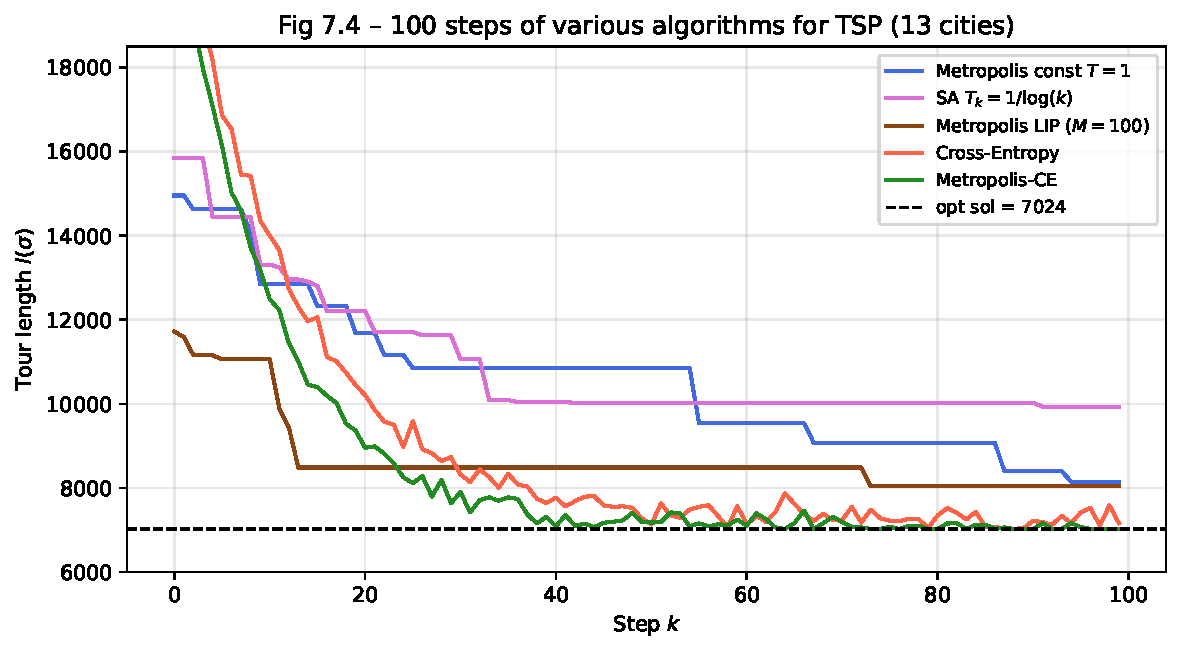
\includegraphics[width=0.64\textwidth]{fig_tsp_comparison}
\end{center}
\small
\textbf{A single representative run} of each algorithm over 100 steps.  The
$y$-axis is the tour length; the dashed line at 7024 is the known optimum.
Plain Metropolis (blue) gets trapped early.  SA (magenta) makes rapid early
progress.  LIP (brown) converges faster due to informed proposals.  CE (red)
and Metropolis-CE (green) both converge very close to the optimum.

\begin{center}
  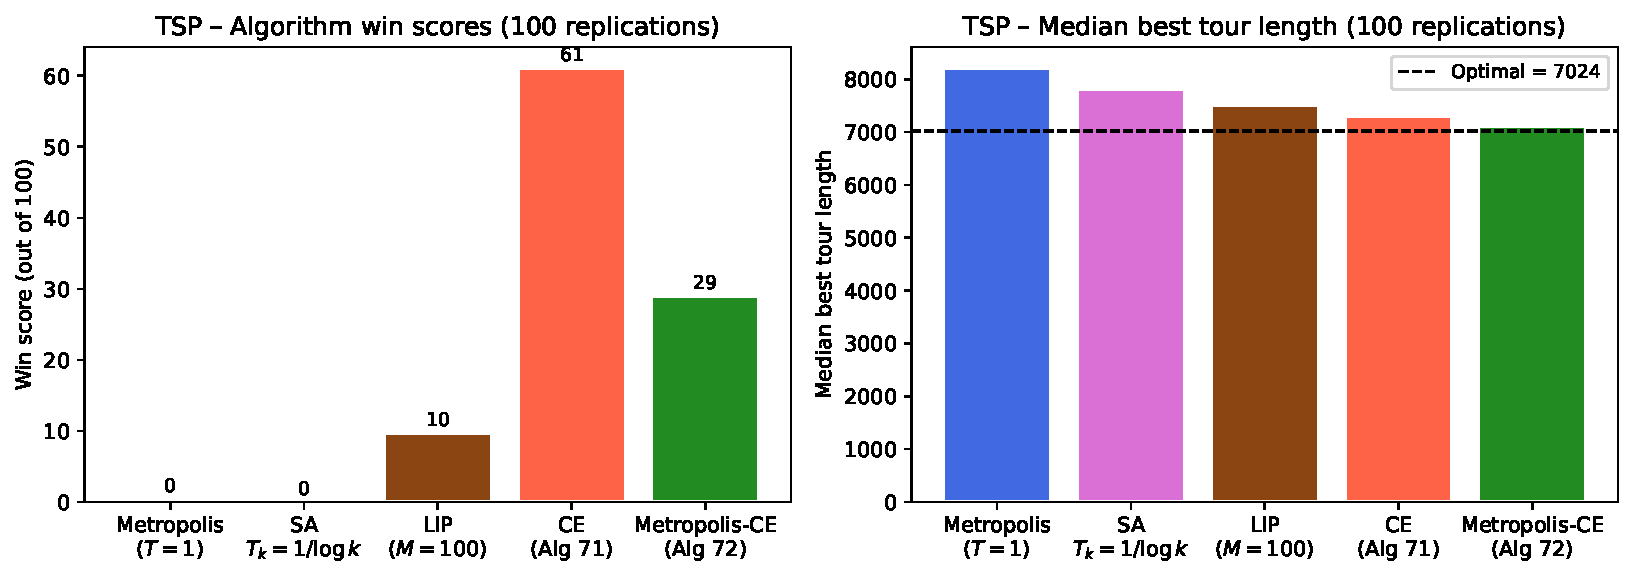
\includegraphics[width=0.48\textwidth]{fig_tsp_results_bar}
\end{center}
\small
\textbf{Win scores across 100 replications.}  CE wins most often (61/100)
but requires $\approx 230$\,s.  Metropolis-CE wins 29 times with only
$\sim 10$\,s --- a $23\times$ speed-up with comparable quality.  LIP
provides a useful middle ground (10\,s, 9.66 wins).

\framebreak

\textbf{7.6.2 The Knapsack Problem ($d=100$)}

For the knapsack ($d=100$, $w_i=i$, $v_i=i^{1.2}$, $W=3000$), all five
algorithms were run 100 times for 100 steps each.

\begin{center}
  \small
  \begin{tabular}{lrr}
    \toprule
    Algorithm & Best value found (typical) & Win score\\
    \midrule
    Metropolis ($T=1$)         & $\sim 6800$ & very low\\
    Gibbs sampler ($T=1$)      & $\sim 6800$ & very low\\
    LIP ($M=100$)              & $\sim 7100$ & moderate\\
    Cross-Entropy              & $\sim 7200$ & high\\
    Metropolis-CE              & $\sim 7400$ & \textbf{100/100}\\
    \bottomrule
  \end{tabular}
\end{center}

Metropolis-CE won \textbf{every single replication} (100/100).  The reason:
the adaptive transition distribution $\btheta$ learns which specific
bit-flips improve the current solution from the current state.  After 50
steps the knapsack is nearly full (weight $\approx 2900$ out of 3000).  The
only profitable moves are to swap a low-value item for a high-value item.
Uninformed Metropolis picks random bits to flip; Metropolis-CE's adaptive
$\btheta$ concentrates probability precisely on these productive swaps,
making nearly every step count.

\begin{alertblock}{Key Takeaways from the Comparison}
  CE and Metropolis-CE outperform all Metropolis-based methods on both
  benchmarks.  Metropolis-CE is $\approx 23\times$ faster than CE on TSP
  with comparable or better solution quality.  LIP offers a useful middle
  ground.  For practical use: start with Metropolis to verify correctness,
  try SA or LIP for better quality, and use CE or Metropolis-CE for the
  highest-quality solutions.
\end{alertblock}

\end{frame}

% ============================================================
\section{7.7 Bibliographical Notes}
% ============================================================

\begin{frame}[allowframebreaks]{7.7 Bibliographical Notes}

The field of stochastic optimisation draws on ideas from statistical
mechanics, combinatorial optimisation, and information theory.

\medskip
\textbf{Metropolis algorithm.}
The Metropolis algorithm was introduced by Metropolis et al.\ (1953) in the
context of statistical mechanics and generalised by Hastings (1970) to the
Metropolis--Hastings form studied in this chapter.  The application to
\textbf{decryption of substitution ciphers} using bigram frequencies is
described in Diaconis [24], which provides an accessible account of
code-breaking via MCMC.

\medskip
\textbf{Simulated Annealing.}
SA was introduced independently by Kirkpatrick, Gelatt \& Vecchi (1983) and
\v{C}ern\'{y} (1985).  The theoretical convergence result under logarithmic
cooling --- the condition $\sum_k e^{-c/T_k} = \infty$ --- is due to
\textbf{Haj\'{e}k [76]}, who proved that SA converges to the global optimum
if and only if this condition holds.

\medskip
\textbf{Locally Informed Proposals.}
LIP is inspired by Zanella (2020) on ``informed proposals for discrete
spaces'' and by MALA (Metropolis-Adjusted Langevin Algorithm) for continuous
distributions.  The specific gradient-based approximation used here is from
\textbf{Grathwohl et al.\ [71]}, \emph{``Oops I Took a Gradient: Scalable
Sampling for Discrete Distributions''}.

\medskip
\textbf{Cross-Entropy method.}
The CE method for optimisation was developed by \textbf{Rubinstein [31]} and
is comprehensively described in Rubinstein \& Kroese, \emph{The
Cross-Entropy Method} (Springer, 2004).

\medskip
\textbf{TSP and the Held--Karp algorithm.}
The Held--Karp dynamic-programming algorithm [82] (Held \& Karp, 1962) runs
in $O(n^2 2^n)$ time and is exact but exponential.  The 13-city distance
matrix was obtained from
\texttt{https://developers.google.com/optimization/routing/tsp}.

\end{frame}

% ============================================================
\section{7.8 Exercises}
% ============================================================

\begin{frame}[allowframebreaks]{7.8 Selected Exercises}

\begin{block}{Exercise 7.L.1 (Substitution Cipher Decryption)}
  Implement the Metropolis-based decryption algorithm for a substitution
  cipher.  Run for 3000 steps from a random permutation.  Report:
  \begin{enumerate}[(a)]
    \item The evolution of log-likelihood $l(\sigma_k)$ over steps.
    \item The decrypted messages at steps 1000, 2000, 3000.
  \end{enumerate}
\end{block}

\begin{block}{Exercise 7.L.2 (Metropolis for Permutation Distributions)}
  Consider the probability distribution on $\mathcal{S}_n$:
  \[
    \pi_\sigma = \frac{1}{z}\lambda^{d(\sigma,\sigma_{\mathrm{id}})},
    \quad \lambda > 0,
    \quad d(\sigma,\sigma') = \frac{1}{n}\sum_{i=1}^n |\sigma(i)-\sigma'(i)|,
  \]
  where $\sigma_{\mathrm{id}} = (1,2,\ldots,n)$ is the identity permutation,
  $\lambda$ (lambda, pronounced ``lam-da'') is a positive parameter, and
  $d(\sigma,\sigma')$ is the normalised $\ell_1$-distance between
  permutations.
  \begin{enumerate}[(a)]
    \item Implement Metropolis using the TSP proposal for $\lambda = 0.75$,
      $n = 52$.  For which values of $\lambda$ is the algorithm applicable?
    \item Repeat using the Kendall $\tau$ (tau, pronounced ``taw'') distance.
    \item Use the 2-opt proposal (Remark~7.2.4) and compare convergence.
  \end{enumerate}
\end{block}

\framebreak

\begin{block}{Exercise 7.L.3 (Fixed-Point Distribution on Permutations)}
  Consider $\pi_\sigma = \lambda^{\mathrm{FP}(\sigma)} / z$, where
  $\mathrm{FP}(\sigma) = \#\{i : \sigma(i) = i\}$ is the number of fixed
  points.  For $n = 52$ and $\lambda \in \{0.1, 0.75, 2\}$: implement
  Metropolis and compare with the acceptance-rejection method.
\end{block}

\begin{block}{Exercise 7.L.4 (Knapsack: Varying Capacity)}
  Re-implement the Gibbs sampler for the knapsack (Algorithm~63) with
  $d=100$, $w_i=i$, $v_i=i^{1.2}$ and capacities $W \in \{50, 500, 1000, 3000\}$.
  \begin{enumerate}[(a)]
    \item For each $W$, estimate the proportion of random binary vectors
      that are feasible.  Compare the best values found by Gibbs vs random
      sampling.
    \item Implement Metropolis for the same problem and compare.
  \end{enumerate}
\end{block}

\begin{block}{Exercise 7.L.5 (Simulated Annealing for Knapsack)}
  Construct an SA version of the knapsack Gibbs sampler:
  \[
    \pi^{T_k}_{\bx} = \frac{\exp(\bv\cdot\bx/T_k)}{z_{T_k}},
    \quad \bw\cdot\bx \le W.
  \]
  Compare for $W \in \{3000, 50\}$: fixed temperature $T_k = 1$ vs
  logarithmic cooling $T_k = 1/\log(k)$.
\end{block}

\framebreak

\begin{block}{Exercise 7.L.6 (CE for TSP: Alternative Parametrisation)}
  In Sect.~7.4 the TSP used a stochastic matrix $\btheta = (\theta_{ij})$
  ($n \times n$).  Consider instead a \emph{vector} parametrisation
  $\btheta = (\theta_1,\ldots,\theta_n)$ (a probability distribution over
  cities).
  \begin{enumerate}[(a)]
    \item Describe formally how to sample a tour from this vector.
    \item Implement the full CE method using both parametrisations for
      $n=13$ and the distance matrix $\mathbf{M}$ from Fig.~7.3.
    \item Compare convergence speed and solution quality.  Does the matrix
      parametrisation capture more structure of the TSP than the vector
      parametrisation?
  \end{enumerate}
\end{block}

\end{frame}

% ============================================================
\section{Chapter Summary}
% ============================================================

\begin{frame}[allowframebreaks]{Chapter 7 Summary}

This chapter covered five Monte Carlo methods for stochastic optimisation of
combinatorial problems.  Each method builds on the Boltzmann distribution as
the bridge between probability and optimisation, but differs in how sampling
is performed.

\begin{block}{Five Methods: Side-by-Side Comparison}
  \small
  \begin{tabular}{p{2.3cm}p{1.8cm}p{4.4cm}p{2.6cm}}
    \toprule
    Method & State & Core mechanism & Key parameters\\
    \midrule
    Metropolis (fixed $T$)
      & single solution
      & Boltzmann stationary dist.\ at fixed $T$
      & $T$, graph $G$\\[4pt]
    Simulated Annealing
      & single solution
      & decrease $T_k \searrow 0$; non-homogeneous MC
      & cooling schedule $\{T_k\}$\\[4pt]
    LIP
      & single solution
      & proposal weighted by $\pi$-ratio; balancing fn $g$
      & $\beta$, $g(\cdot)$, $M$\\[4pt]
    Cross-Entropy
      & distribution $\btheta$
      & MLE update over elite samples; $\gamma_t \nearrow$
      & $M$, $\rho$, $\alpha$\\[4pt]
    Metropolis-CE
      & solution + distribution
      & CE update of the transition distribution
      & all of the above\\
    \bottomrule
  \end{tabular}
\end{block}

\framebreak

\textbf{Theoretical guarantees.}

Metropolis at fixed $T$ has stationary distribution $\pi^T$ (the Boltzmann
distribution).  The mode of $\pi^T$ is the minimiser of $H$.  No
convergence guarantee for finite runs; the chain may remain trapped in local
minima.

Simulated Annealing converges to the global optimum $D^*$ with probability
1 if and only if the cooling satisfies $\sum_k e^{-c/T_k} = \infty$
(Haj\'{e}k's condition).  Logarithmic cooling $T_k = d/\log(k)$ satisfies
this; geometric cooling does not.  SA is the only algorithm in this chapter
with a provable global convergence guarantee.

LIP has the same stationary distribution as Metropolis (the Boltzmann
$\pi^T$), but explores more efficiently by using local gradient information.
No additional convergence guarantees beyond standard Metropolis.

CE and Metropolis-CE are heuristic algorithms with no general convergence
guarantees, but empirically the most effective on both benchmarks studied.

\medskip
\textbf{Practical recommendations.}
\begin{enumerate}
  \item Start with plain Metropolis to verify implementation correctness and
    understand the problem landscape.
  \item If Metropolis gets trapped: try SA with geometric cooling
    $T_k = 0.99^k T_0$.
  \item For better quality with moderate budget: try LIP (better solutions,
    $\sim M\times$ more expensive per step).
  \item For best solution quality with larger budget: use CE or
    Metropolis-CE.  CE provides the richest distributional model but is
    slowest; Metropolis-CE is $\approx 20\times$ faster with comparable
    quality.
\end{enumerate}

\begin{alertblock}{Unifying Theme: Probability as a Search Tool}
  All five methods use the Boltzmann distribution as a bridge between
  probability and optimisation.  The core principle: assign higher
  probability to better solutions, then \emph{sample} efficiently from that
  distribution.  The methods differ only in how they implement this sampling,
  trading off computational cost per step against the quality of exploration.
\end{alertblock}

\end{frame}

\end{document}
